%%%%%%%%%%%%%%%%%%%%%%%%%%%%%%%%%%%%%%%%%
% Short Sectioned Assignment LaTeX Template Version 1.0 (5/5/12)
% This template has been downloaded from: http://www.LaTeXTemplates.com
% Original author:  Frits Wenneker (http://www.howtotex.com)
% License: CC BY-NC-SA 3.0 (http://creativecommons.org/licenses/by-nc-sa/3.0/)
%%%%%%%%%%%%%%%%%%%%%%%%%%%%%%%%%%%%%%%%%

%----------------------------------------------------------------------------------------
%	PACKAGES AND OTHER DOCUMENT CONFIGURATIONS
%----------------------------------------------------------------------------------------

\documentclass[paper=a4, fontsize=11pt]{scrartcl} % A4 paper and 11pt font size

% ---- Entrada y salida de texto -----
\usepackage{listings}
\usepackage[T1]{fontenc} % Use 8-bit encoding that has 256 glyphs
\usepackage[utf8]{inputenc}
%\usepackage{fourier} % Use the Adobe Utopia font for the document - comment this line to return to the LaTeX default

% ---- Idioma --------

\usepackage{svg}
\usepackage{amsmath}
\usepackage[spanish, es-tabla]{babel} % Selecciona el español para palabras introducidas automáticamente, p.ej. "septiembre" en la fecha y especifica que se use la palabra Tabla en vez de Cuadro

% ---- Otros paquetes ----

\usepackage{url} % ,href} %para incluir URLs e hipervínculos dentro del texto (aunque hay que instalar href)
\usepackage{amsmath,amsfonts,amsthm} % Math packages
%\usepackage{graphics,graphicx, floatrow} %para incluir imágenes y notas en las imágenes
\usepackage{graphics,graphicx, float} %para incluir imágenes y colocarlas

% Para hacer tablas comlejas
%\usepackage{multirow}
%\usepackage{threeparttable}

%\usepackage{sectsty} % Allows customizing section commands
%\allsectionsfont{\centering \normalfont\scshape} % Make all sections centered, the default font and small caps

\usepackage{fancyhdr} % Custom headers and footers
\pagestyle{fancyplain} % Makes all pages in the document conform to the custom headers and footers
\fancyhead{} % No page header - if you want one, create it in the same way as the footers below
\fancyfoot[L]{} % Empty left footer
\fancyfoot[C]{} % Empty center footer
\fancyfoot[R]{\thepage} % Page numbering for right footer
\renewcommand{\headrulewidth}{0pt} % Remove header underlines
\renewcommand{\footrulewidth}{0pt} % Remove footer underlines
\setlength{\headheight}{13.6pt} % Customize the height of the header

\numberwithin{equation}{section} % Number equations within sections (i.e. 1.1, 1.2, 2.1, 2.2 instead of 1, 2, 3, 4)
\numberwithin{figure}{section} % Number figures within sections (i.e. 1.1, 1.2, 2.1, 2.2 instead of 1, 2, 3, 4)
\numberwithin{table}{section} % Number tables within sections (i.e. 1.1, 1.2, 2.1, 2.2 instead of 1, 2, 3, 4)

\setlength\parindent{0pt} % Removes all indentation from paragraphs - comment this line for an assignment with lots of text

\newcommand{\horrule}[1]{\rule{\linewidth}{#1}} % Create horizontal rule command with 1 argument of height


%----------------------------------------------------------------------------------------
%	TÍTULO Y DATOS DEL ALUMNO
%----------------------------------------------------------------------------------------

\title{	
\normalfont \normalsize 
\textsc{\textbf{Ingeniería de Servidores (2016-2017)} \\ Grado en Ingeniería Informática \\ Universidad de Granada} \\ [25pt] % Your university, school and/or department name(s)
\horrule{0.5pt} \\[0.4cm] % Thin top horizontal rule
\huge Memoria Práctica 3 \\ % The assignment title
\horrule{2pt} \\[0.5cm] % Thick bottom horizontal rule
\begin{figure*}[!ht]
	\begin{center}
		
\includegraphics[width=0.7\textwidth]{imagenes/escudo-de-la-universidad-de-granada}
	\end{center}
\end{figure*}
}

\author{Iván Rodríguez Millán} % Nombre y apellidos

\date{\normalsize\today} % Incluye la fecha actual

%----------------------------------------------------------------------------------------
% DOCUMENTO
%----------------------------------------------------------------------------------------

\begin{document}

\maketitle % Muestra el Título

\newpage %inserta un salto de página

\tableofcontents % para generar el índice de contenidos

\listoffigures

\listoftables

\newpage

\section{?`Qué archivo le permite ver qué programas se han instalado con el gestor de paquetes? ?`Qué significan las terminaciones .1.gz o .2.gz de los archivos en ese directorio?}
\subsection{Respuesta A):}

En el caso de Ubuntu Server, en donde usamos el gestor de paquetes apt, el archivo en donde se puede ver el historial de los programas que se han instalado es ``/var/log/apt/history.log''. \cite{debianAPTLOG}

\begin{figure}[H]
	\begin{center}
		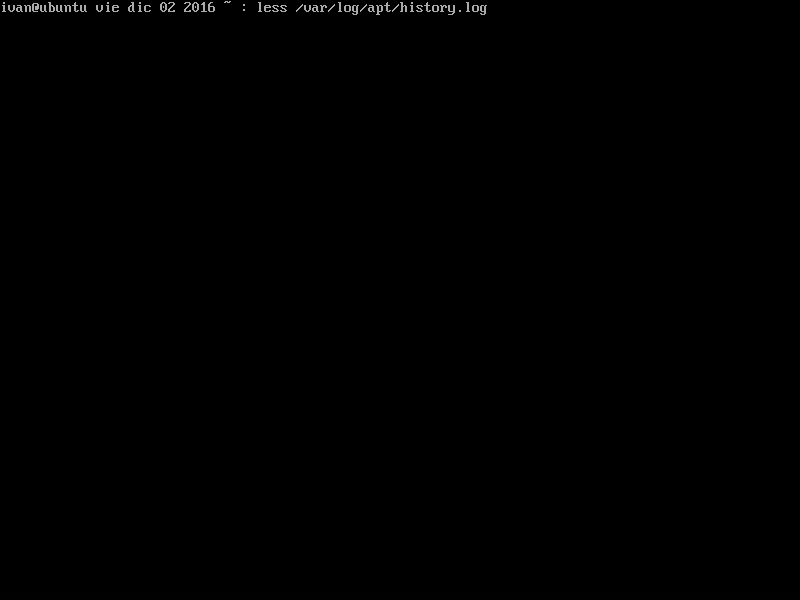
\includegraphics[width=0.7\textwidth]{Imagenes/Comando_acceso_historial_apt}
		\caption{Comando para acceder de forma cómo al fichero con el historial del gestor APT.} \label{fig:1}
	\end{center}
\end{figure}

\begin{figure}[H]
	\begin{center}
		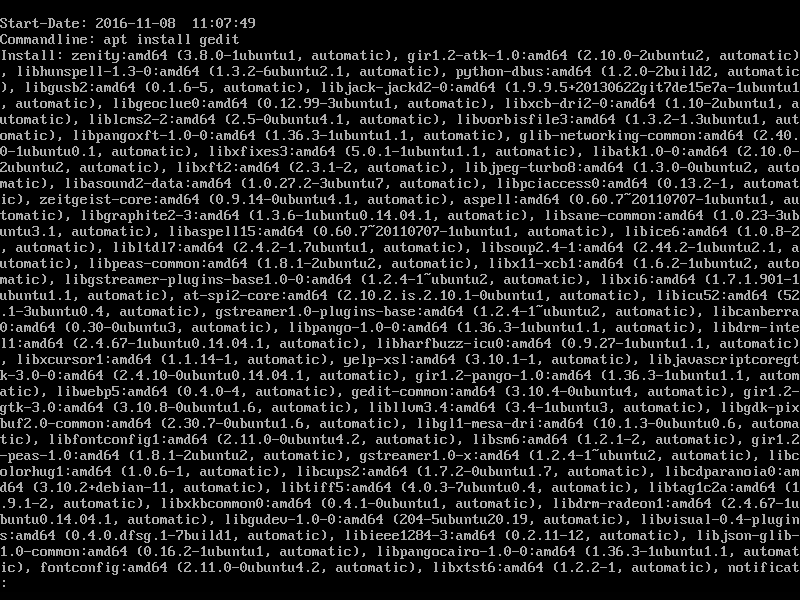
\includegraphics[width=0.7\textwidth]{Imagenes/Instalacion_gedit_server}
		\caption{Ejemplo del fichero history.log, mostrando información sobre la instalación de gedit.} \label{fig:2}
	\end{center}
\end{figure}

Mientras que en el caso de CentOS 7, al usar el gestor de paquetes yum, el archivo es ``/var/log/yum.log''. \cite{RedHatAPTLOG}

\begin{figure}[H]
	\begin{center}
		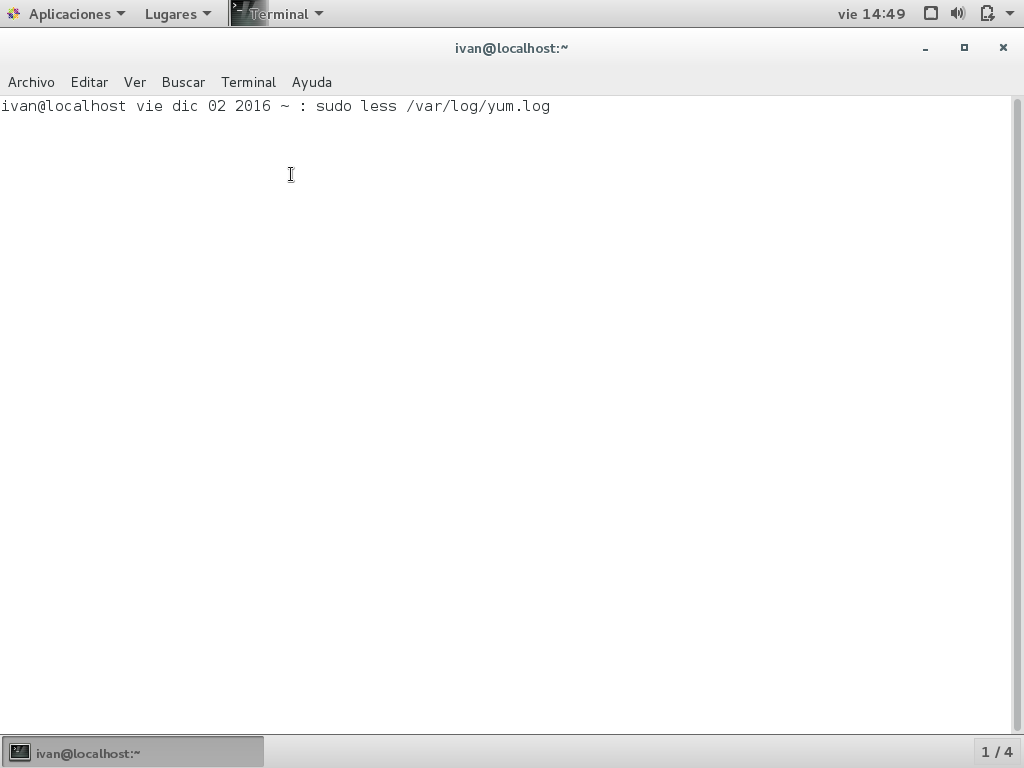
\includegraphics[width=0.7\textwidth]{Imagenes/Comando_acceso_yum_log}
		\caption{Comando para acceder de forma cómo al fichero con el historial del gestor YUM.} \label{fig:3}
	\end{center}
\end{figure}

\begin{figure}[H]
	\begin{center}
		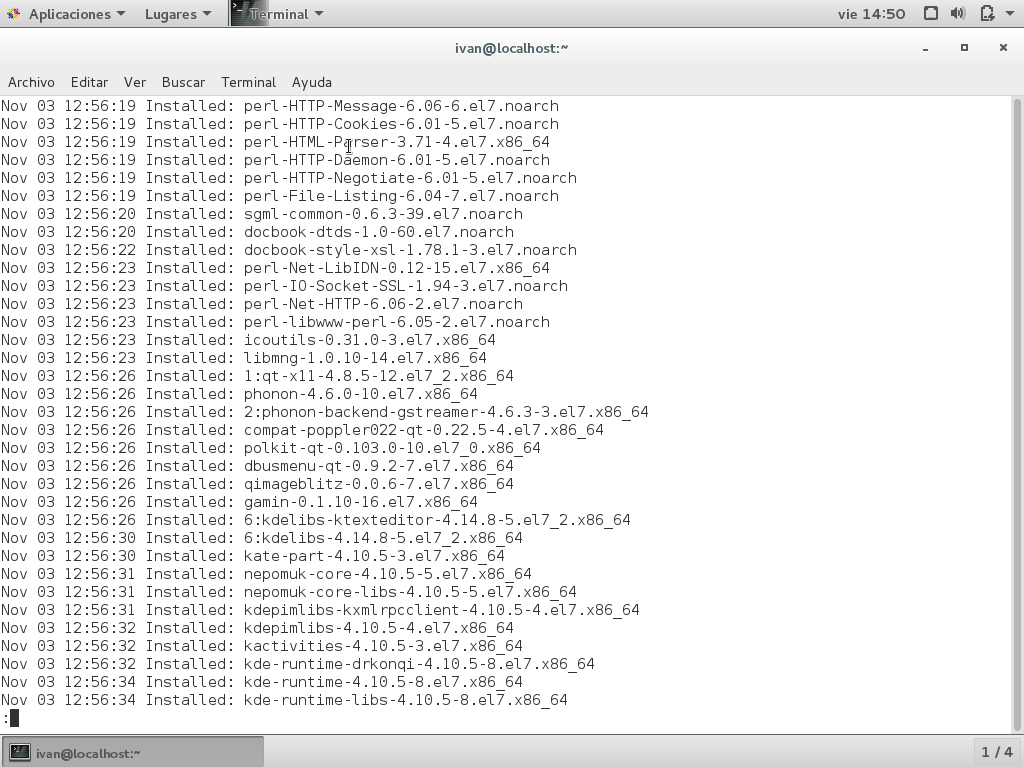
\includegraphics[width=0.7\textwidth]{Imagenes/Fichero_yum_log}
		\caption{Ejemplo del fichero yum.log} \label{fig:4}
	\end{center}
\end{figure}

\subsection{Respuesta B):}

Dado que el sistema puede llegar a generar ficheros log demasiado extensos, y por lo tanto crear serios inconvenientes en el almacenamiento de nuestro servidor, existe un demonio cron (cron.daily)\cite{CRON.DAILY} , que todos los días ejecuta un script (logrotate) que permite automatizar la rotación, compresión, borrado y envío de ficheros log. \cite{Logrotate}

Así pues respondiendo a la pregunta el script ``logrotate'' los comprime con la extension ``nº.gz'' , así cuanto mayor sea el número más viejo será el archivo.\cite{FILElogs}

\section{?`Qué archivo ha de modificar para programar una tarea? Escriba la línea necesaria para ejecutar una vez al día una copia del directorio home/ivan/codigo a  home/ivan/seguridad/\$fecha donde \$fecha es la fecha actual(puede usar el comando date).}
\subsection{Respuesta : }
Si se quiere programar una tarea se tienen dos opciones, o bien modificar el archivo /etc/crontab ó escribir archivos crontab adicionales en el directorio /etc/cron.d . \cite{CRONTAB}

A continuación se muestra un ejemplo de como realizar una copia de seguridad de un directorio codigo a otro directorio seguridad y dentro de seguridad ir guardando todos los días por fecha de copia.

\begin{figure}[H]
	\begin{center}
		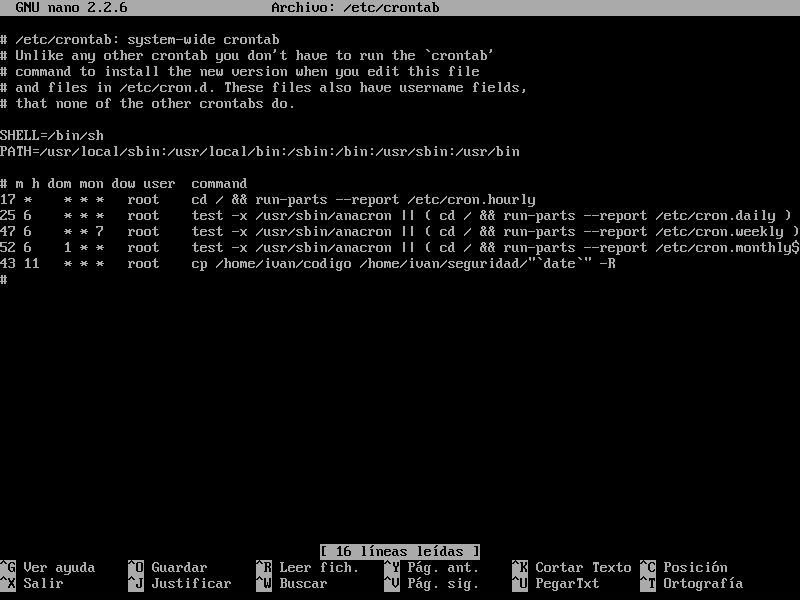
\includegraphics[width=0.7\textwidth]{Imagenes/Crontab_copia_seguridad}
		\caption{Fichero crontab} \label{fig:5}
	\end{center}
\end{figure}

\section{Pruebe a ejecutar el comando dmesg, conectar un dispositivo USB y vuelva a ejecutar el comando. Copie y pegue la salida del comando. (Considere usar dmesg | tail). Comente qué observa en la información mostrada.}
\subsection{Respuesta : }
El comando dmesg \cite{DMESG} es usado para examinar las señales del kernel.
En nuestro caso vamos a comprobar el funcionamiento del comando viendo las diferencias de no tener insertado un USB a si tenerlo insertado.

\begin{figure}[H]
	\begin{center}
		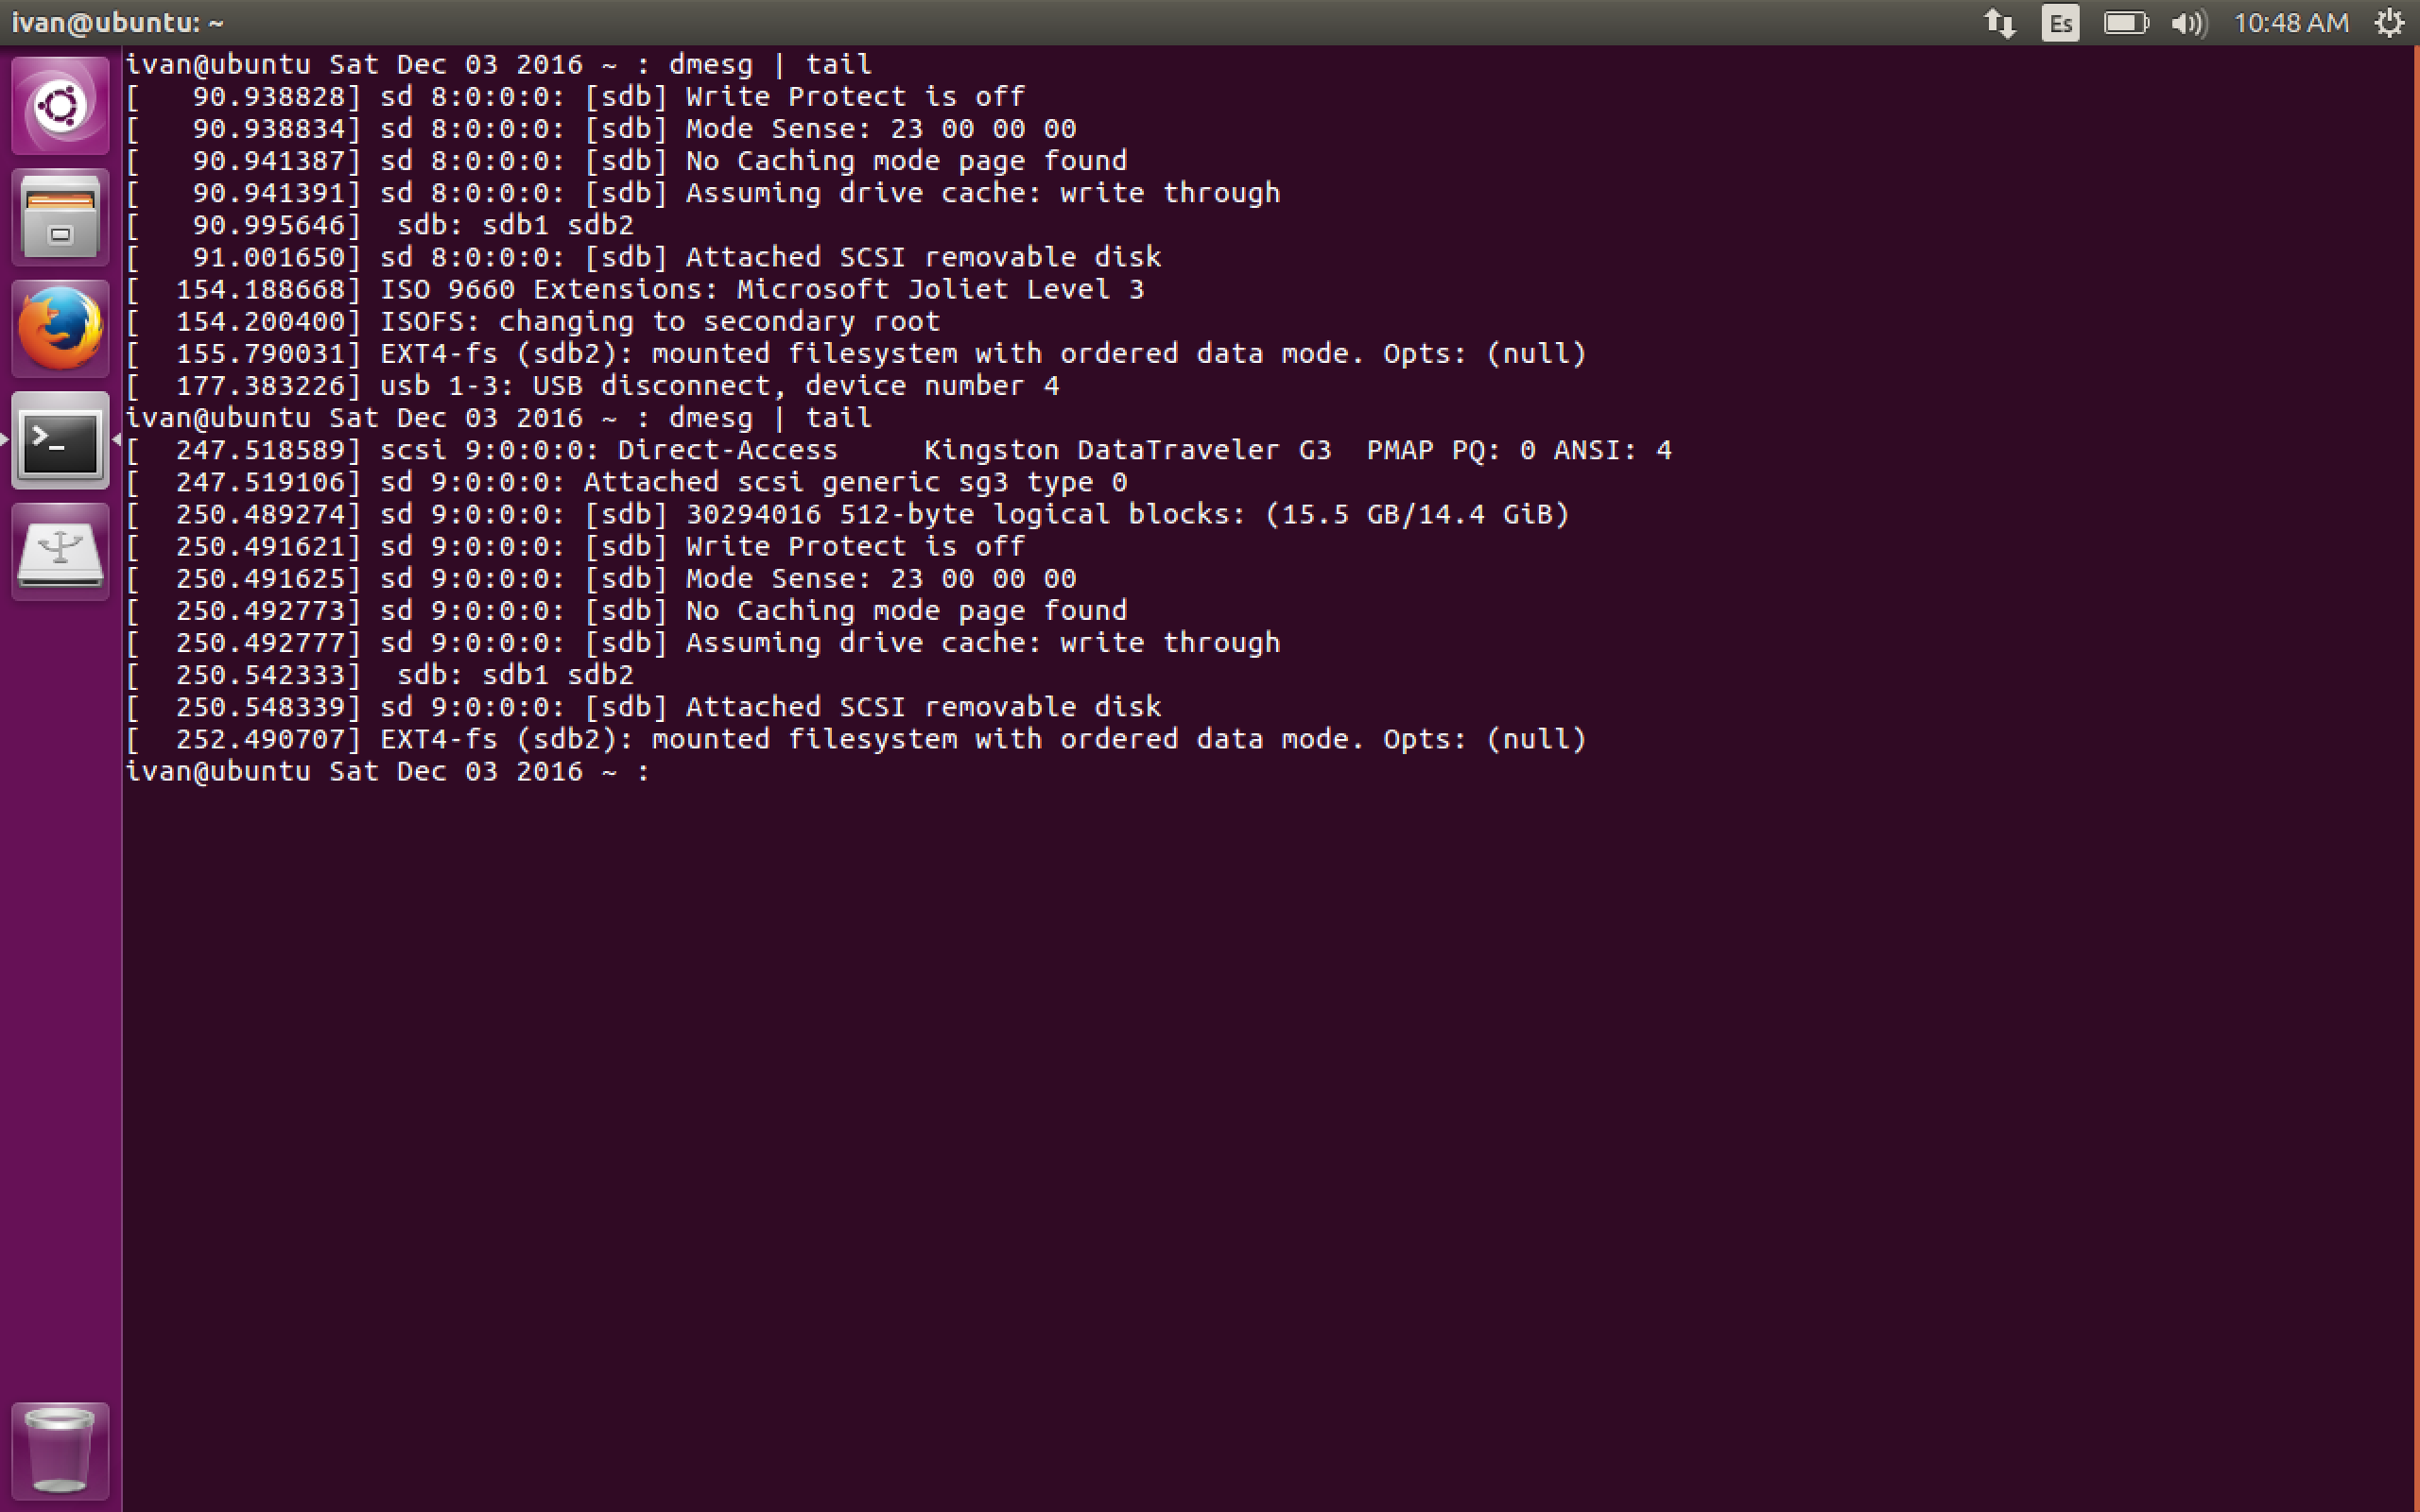
\includegraphics[width=0.7\textwidth]{Imagenes/Diferencia_USB_dmesg}
		\caption{Aplicamos el comando dmesg | tail, para ver las diferencias de tener un USB insertado a no tenerlo.} \label{fig:6}
	\end{center}
\end{figure}

En la imagen de arriba se aplica el comando en primer lugar sin el USB insertado, y en segundo lugar con el USB insertado. Se puede apreciar como nos muestra la marca del USB en este caso Kingston. Nos muestra también el controlador SCSI(Small computer system interface)
Más abajo nos muestra también la memoria que posee el dis, positivo en Gigas. También nos indica el sistema de archivos que tiene el dispositivo (EXT4).

También tenemos otro comando como dmesg | grep -i USB, para mostrar información de los dispositivos USB entre otros. En donde por ejemplo se nos muestra el numero de serie del dispositivo, marca del dispositivo, tipo de producto (DataTraveler G3).

A parte también se nos muestra información por ejemplo de la CAM(FaceTime HD Camera).

\begin{figure}[H]
	\begin{center}
		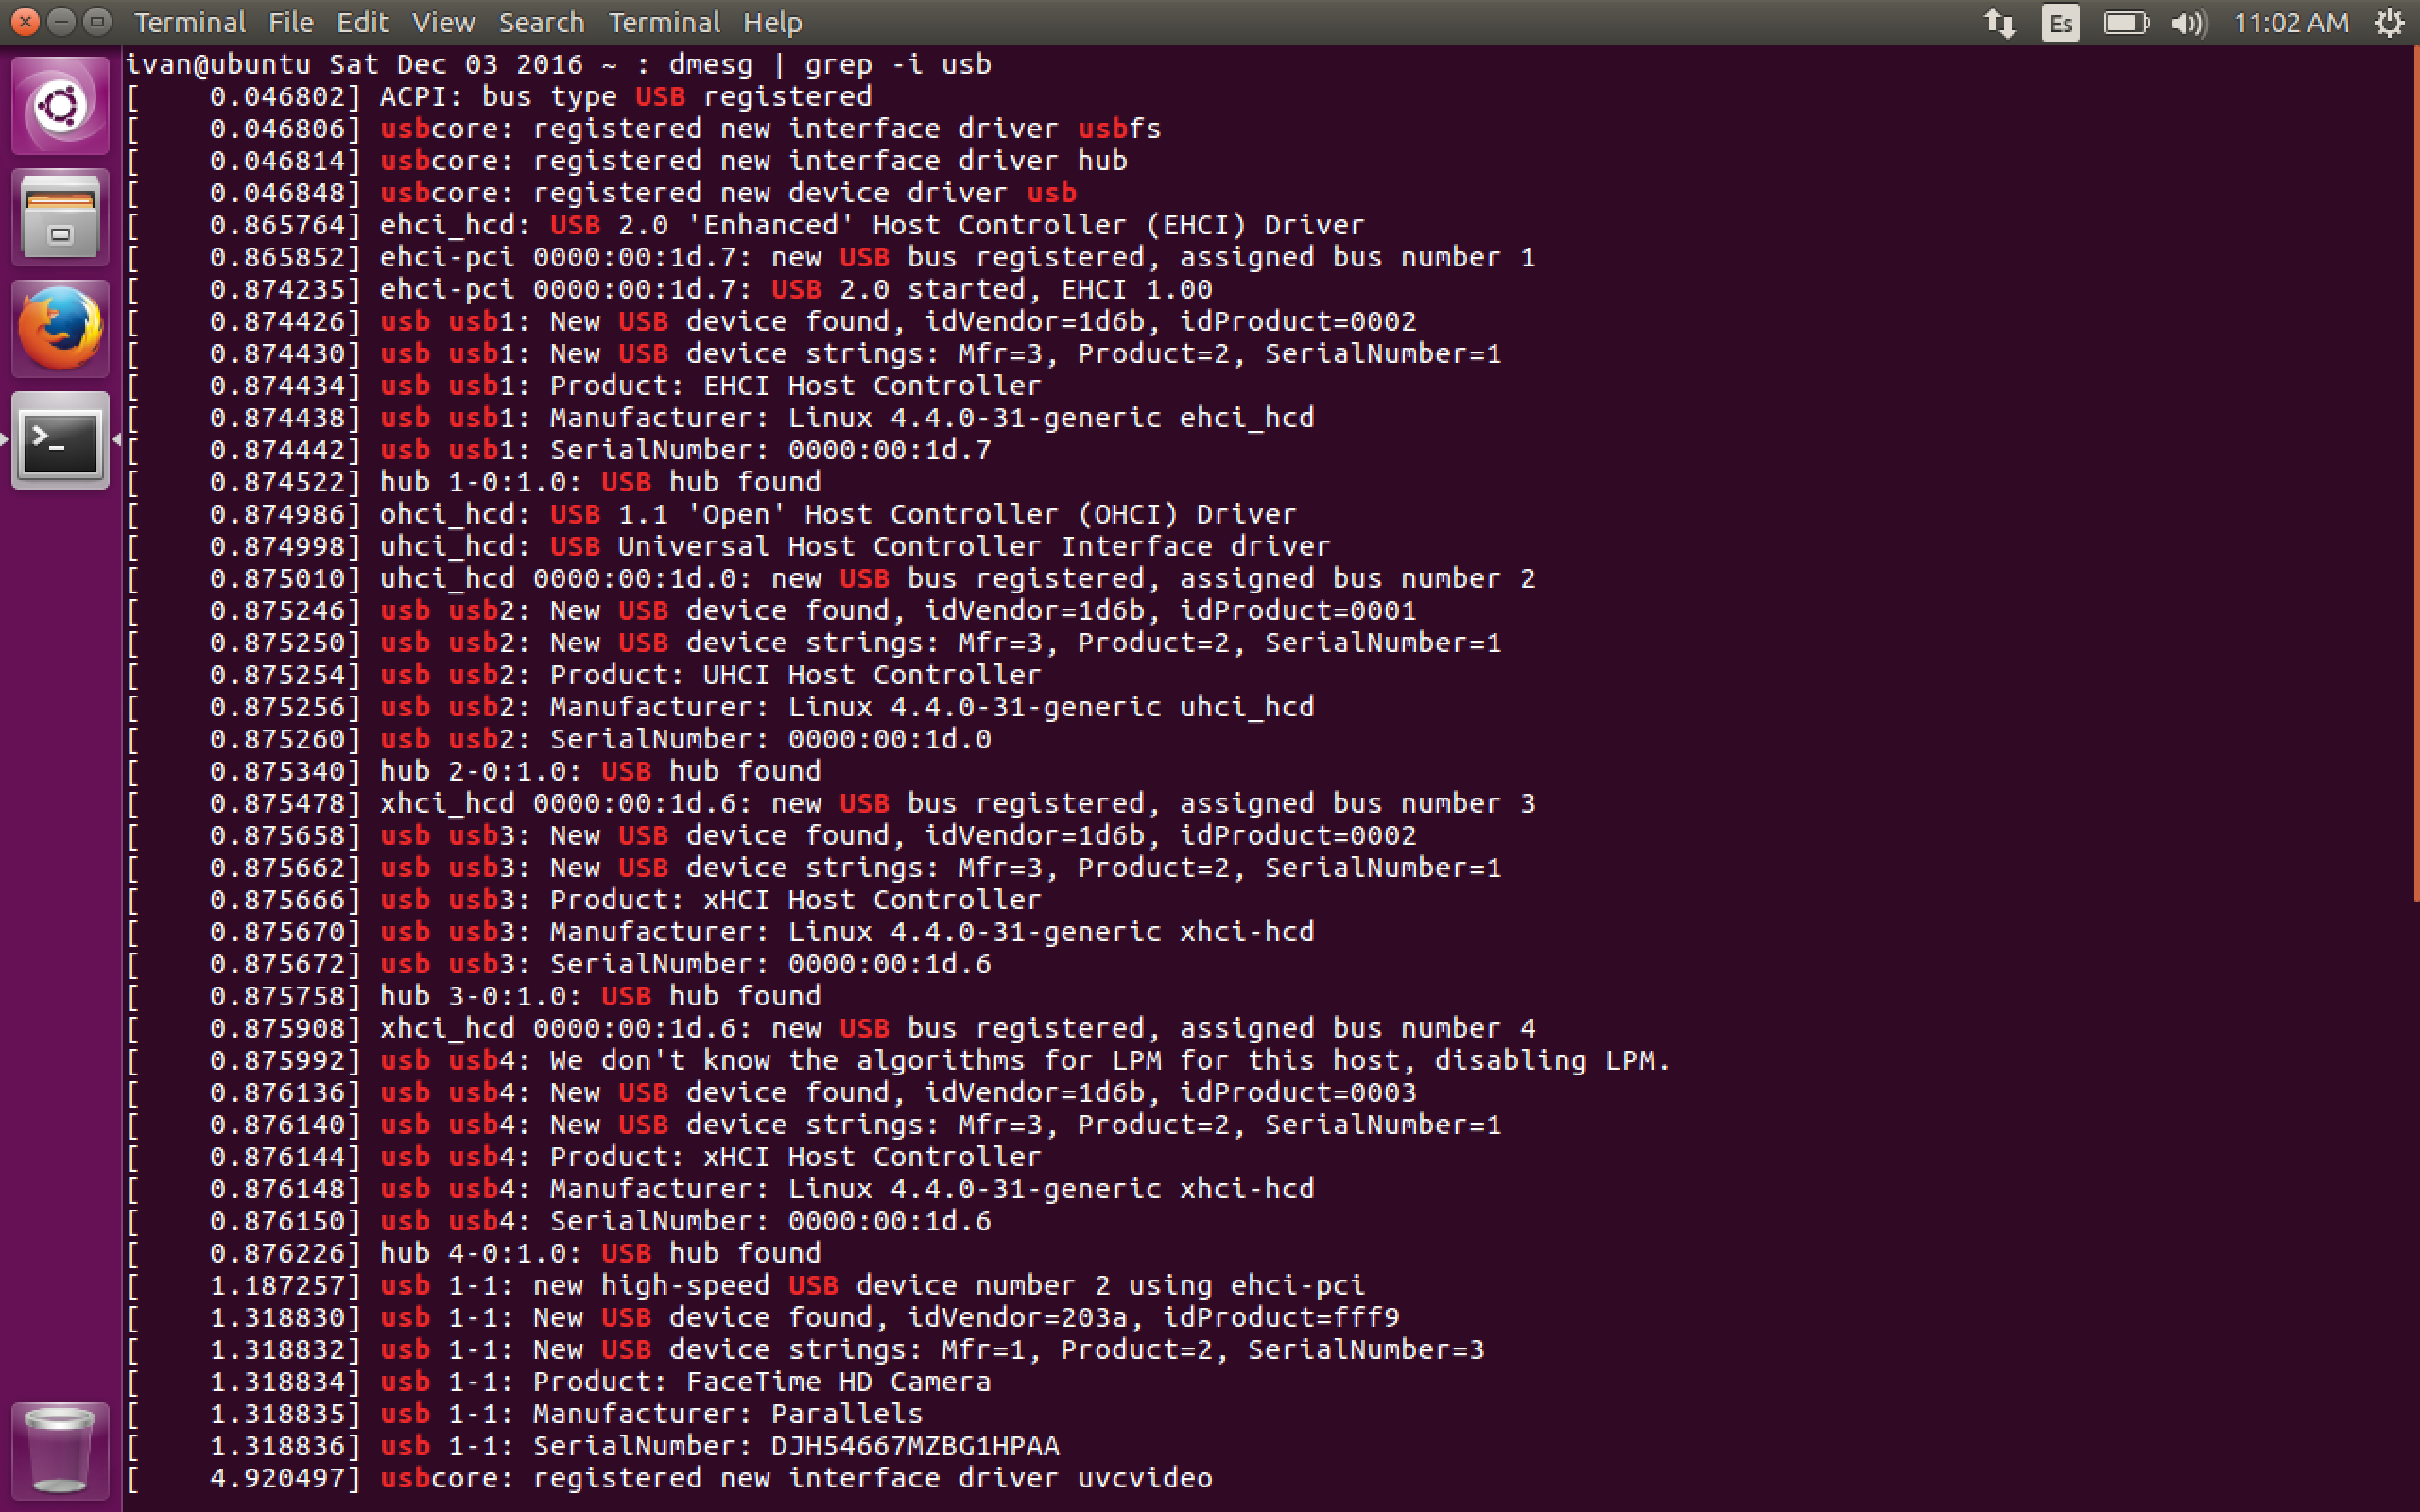
\includegraphics[width=0.7\textwidth]{Imagenes/Comando_dmesg_usb}
		\caption{Aplicamos el comando dmesg | grep -i USB.} \label{fig:7}
	\end{center}
\end{figure}

\begin{figure}[H]
	\begin{center}
		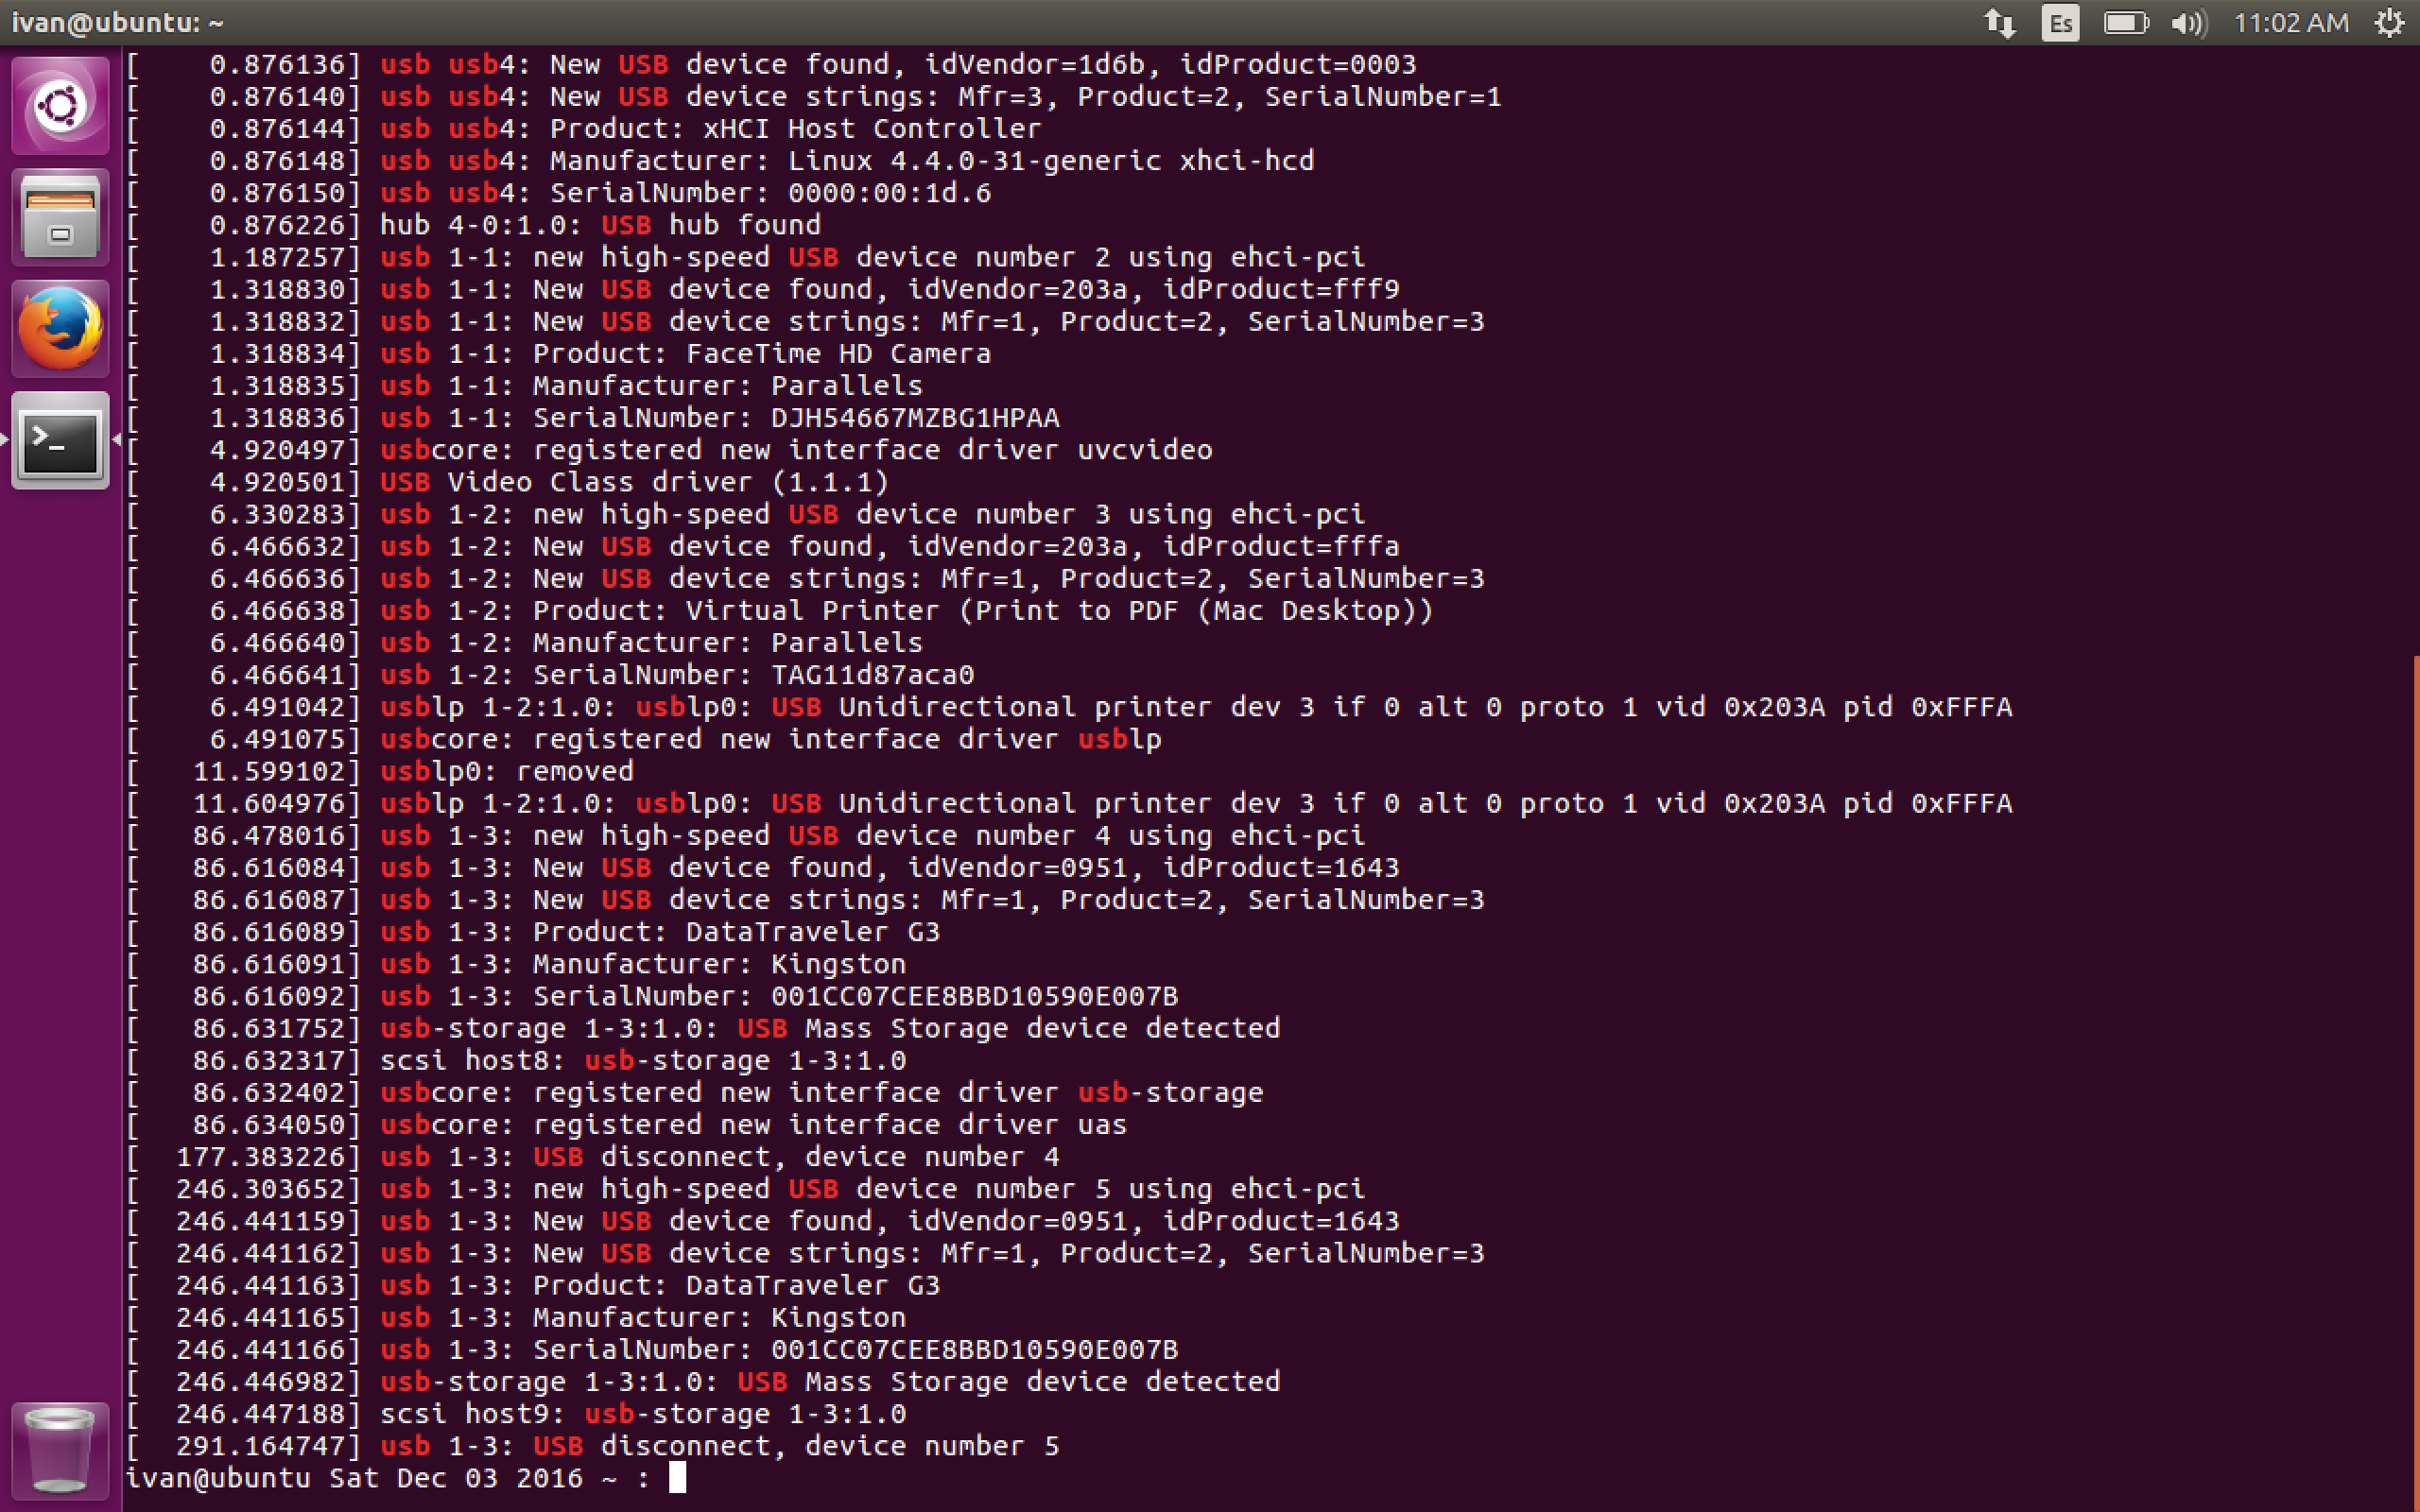
\includegraphics[width=0.7\textwidth]{Imagenes/Comando_dmesg_usb_2}
		\caption{Continuación del comando dmesg | grep -i USB.} \label{fig:7}
	\end{center}
\end{figure}
\newpage
\section{Ejecute el monitor de ``System Performance'' y muestre el resultado. Incluya capturas de pantalla comentando la información que aparece.}
\subsection{Respuesta : }

En primer lugar entramos al monitor Perform, y una vez dentro y en la pestaña de herramientas de monitorización, nos encontramos con el performance monitor, que básicamente consiste en un monitor en tiempo real. Lo primero que nos encontramos es que se realiza una monitorización del porcentaje del procesador. \newline

\begin{figure}[H]
	\begin{center}
		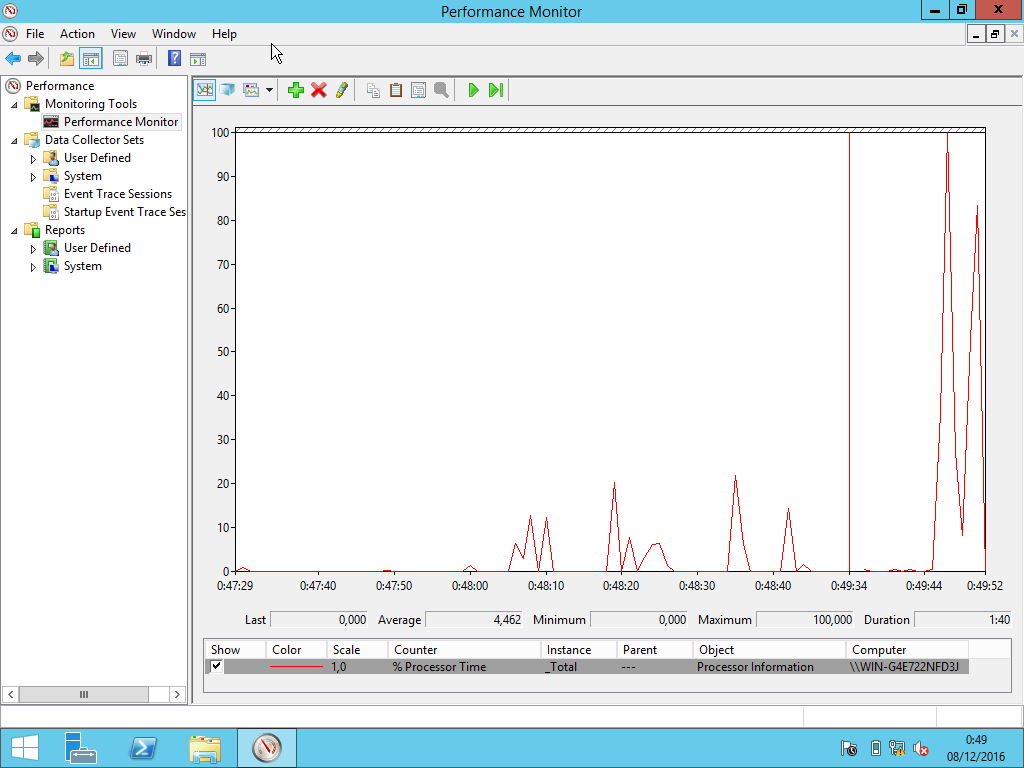
\includegraphics[width=0.7\textwidth]{Imagenes/Monitorizacion_cpu}
		\caption{Monitorización en tiempo real del porcentaje de procesador usado.} \label{fig:40}
	\end{center}
\end{figure}

A esto le podemos añadir tantos datos como queramos, para ello simplemente debemos irnos a la cruz verde, y añadir los datos a medir. Probamos a introducir datos referentes a la memoria.

\begin{figure}[H]
	\begin{center}
		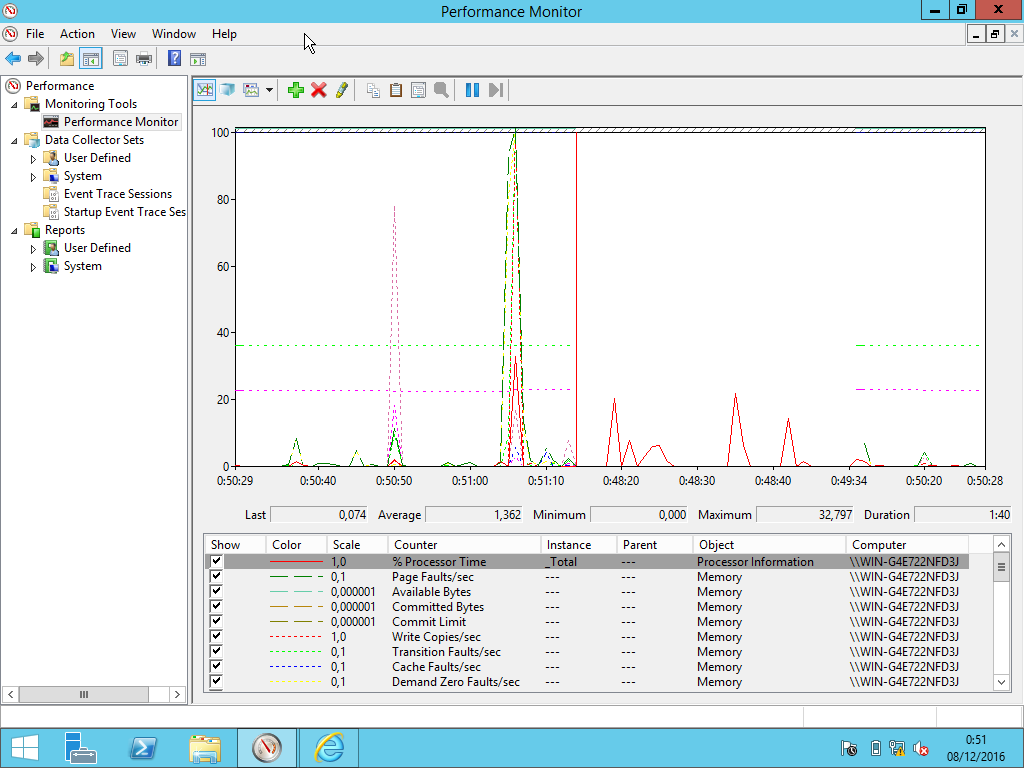
\includegraphics[width=0.7\textwidth]{Imagenes/Monitorizacion_cpu_y_memoria}
		\caption{Monitorización en tiempo real del porcentaje de procesador usado, y memoria.} \label{fig:41}
	\end{center}
\end{figure}

Y comprobamos, que por ejemplo se produce un pico (Línea discontinua en verde), este pico se produce justo cuando abrimos el explorador, hace referencia a una falta de página. \\
\newline
Junto con el pico de la falta de página, también se percibe aunque en menor medida, una pequeña subida en el porcentaje de uso del procesador (como es normal al iniciarse cualquier proceso en el sistema). \\ 
\newline
A continuación se muestra un ejemplo de ejecución de un recopilador de datos. 

En nuestro caso lanzamos el recopilador de datos generado por el sistema (System Performance). Tras esperar 60 segundos, nos muestra los datos recopilados, que en nuestro caso son los siguientes:

\begin{figure}[H]
	\begin{center}
		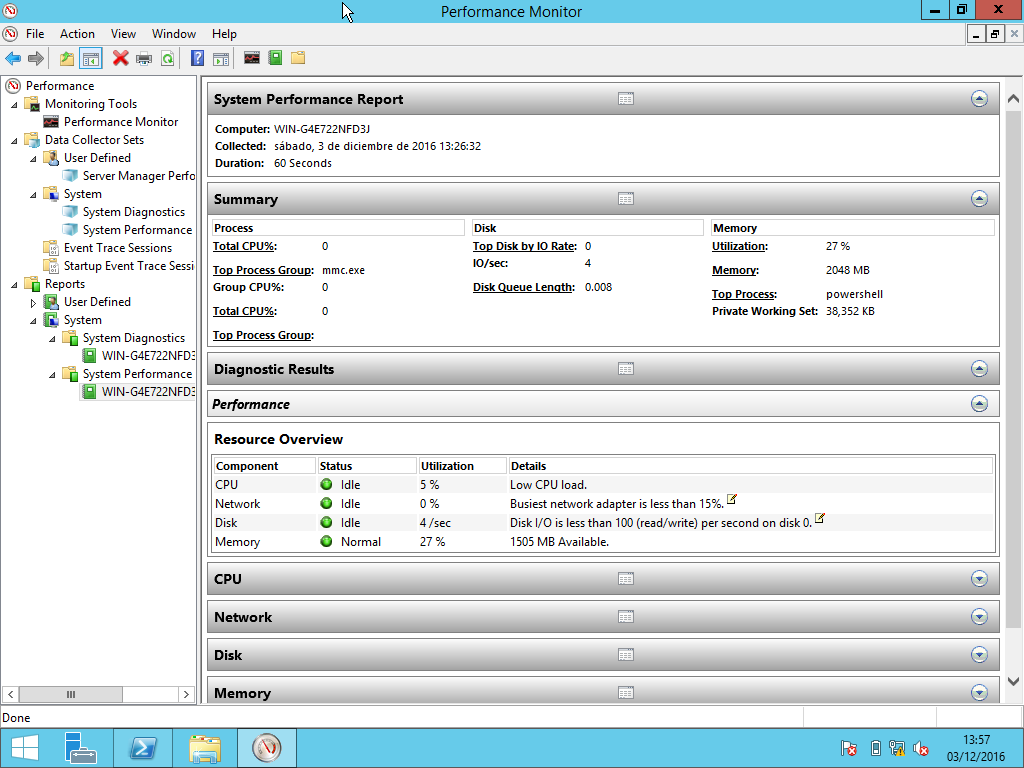
\includegraphics[width=0.7\textwidth]{Imagenes/Datos_recopilados_del_diagnostico}
		\caption{Datos recopilados del diagnóstico realizado mediante el system performance.} \label{fig:8}
	\end{center}
\end{figure}

En primer lugar se nos muestra un sumario con datos del procesador, disco y memoria. Si pulsamos en el texto mas inferior que detalla algo de información, vemos que nos lleva a otra parte en donde nos detalla perfectamente todo. Por ejemplo para el caso de la CPU:
\begin{figure}[H]
	\begin{center}
		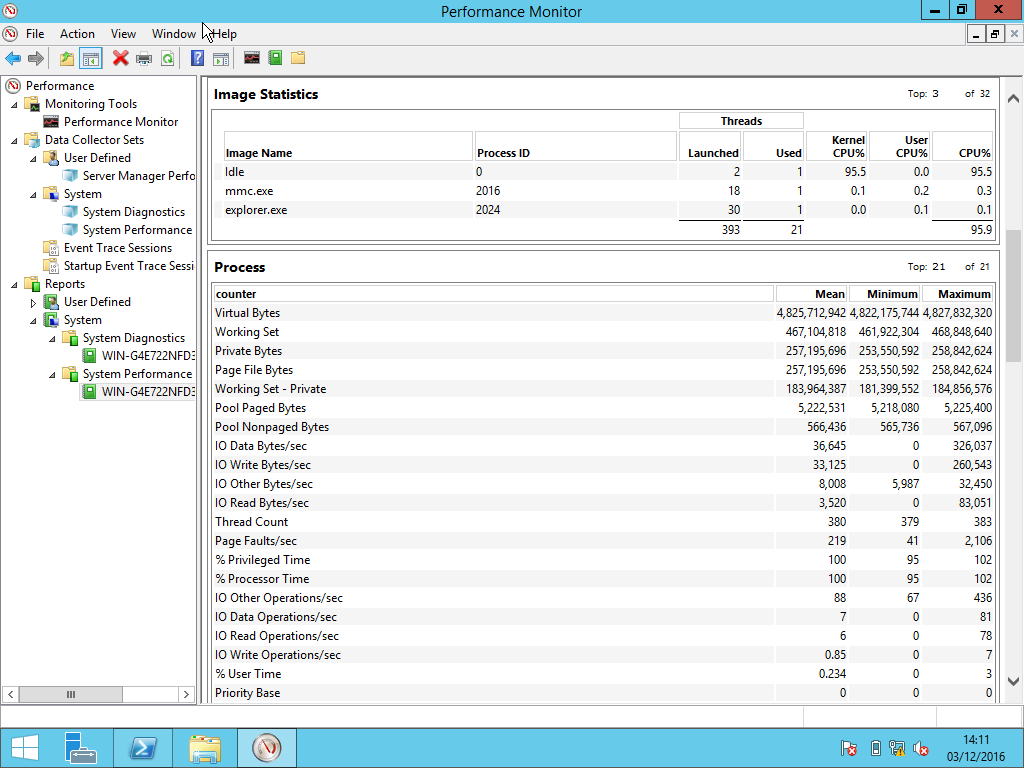
\includegraphics[width=0.7\textwidth]{Imagenes/Desglose_CPU}
		\caption{Desglose de información con respecto al procesador(CPU).} \label{fig:9}
	\end{center}
\end{figure}

Vemos como nos muestran los procesos acompañados de su ID, que han usado la CPU , y el porcentaje de esta que han usado. También vemos las hebras que se han lanzado y se han usado. Así como también se puede observar el porcentaje de CPU del kernel y del usuario para cada proceso.
Se puede observar como el idle(ocioso) se lleva el 95.5\% de porcentaje de CPU, por ello podemos admitir que el sistema está prácticamente inactivo.

Por otro lado y dirigiéndonos a la imagen \ref{fig:8} observamos que la memoria esta en un 27\% de utilización, del total de 2GiB.

Más abajo el propio recopilador de datos nos informa sobre el uso de los principales componentes del servidor como la CPU, la red, la memoria y el disco. Y nos deja caer información como el poco uso de la CPU, el prácticamente nulo uso de la red debido a ese 0\%, en disco el número de entradas/salidas (escritura/lectura) es de 4 por segundo, y en memoria el uso es más normal con unos 1505 MiB disponibles del total de 2GiB.

El recopilador también nos trae una gráfica con muchísimas componentes.

\begin{figure}[H]
	\begin{center}
		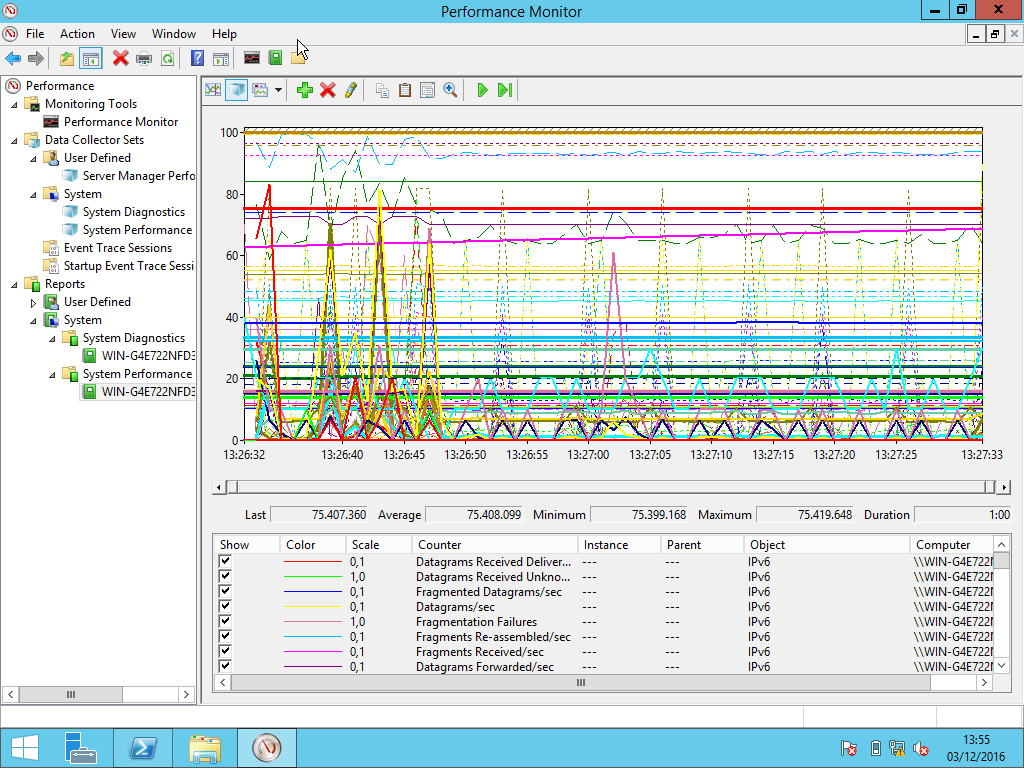
\includegraphics[width=0.7\textwidth]{Imagenes/Grafico_del_diagnostico}
		\caption{Gráfica de los datos recopilados.} \label{fig:10}
	\end{center}
\end{figure}

Como bien se puede apreciar en la imagen la gráfica es poco legible, debido a la cantidad de componentes que se introducen en ella, pero hay una opción para llevarnos esta gráfica a datos, y así poder razonar sobre ellos.

Por ejemplo podemos mostrar los datos sobre la memoria, en ella se puede ver los Bytes disponibles, los KiloBytes disponibles y los MegaBytes disponibles. También los Bytes de cache, las faltas de páginas por segundo, el porcentaje de Bytes en uso, las entradas en las tablas de páginas libres del sistema, etc:

\begin{figure}[H]
	\begin{center}
		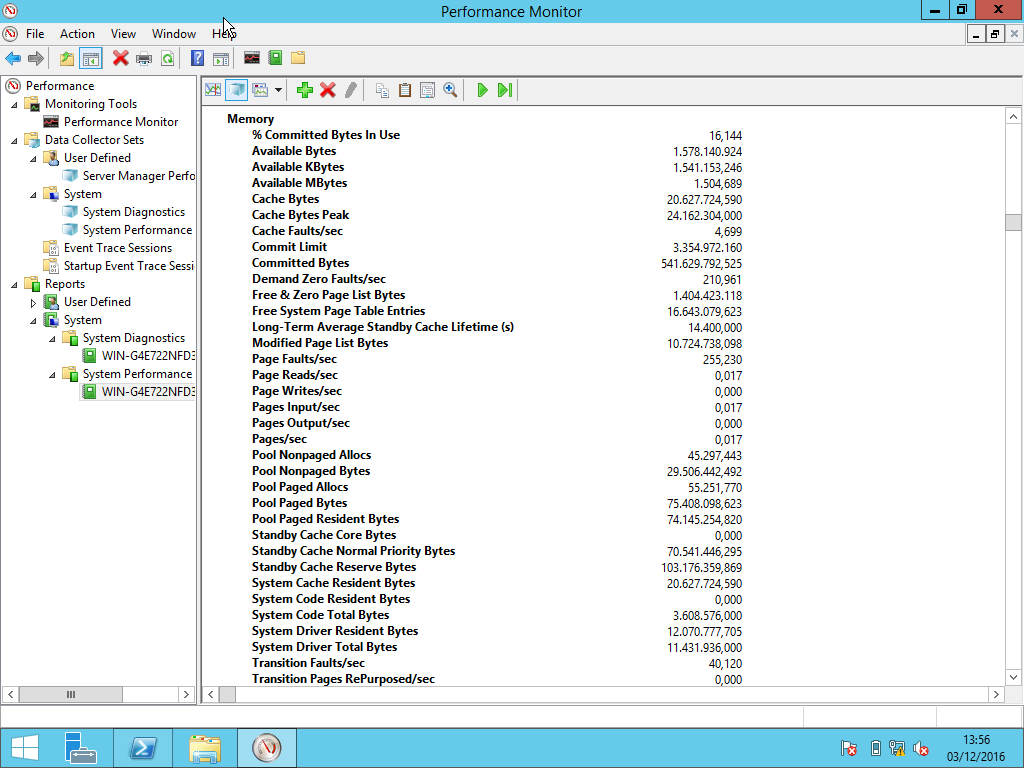
\includegraphics[width=0.7\textwidth]{Imagenes/Datos_grafico_diagnostico}
		\caption{Datos sobre la memoria recopilados.} \label{fig:11}
	\end{center}
\end{figure}

También podemos mostrar información sobre los procesos:
\begin{figure}[H]
	\begin{center}
		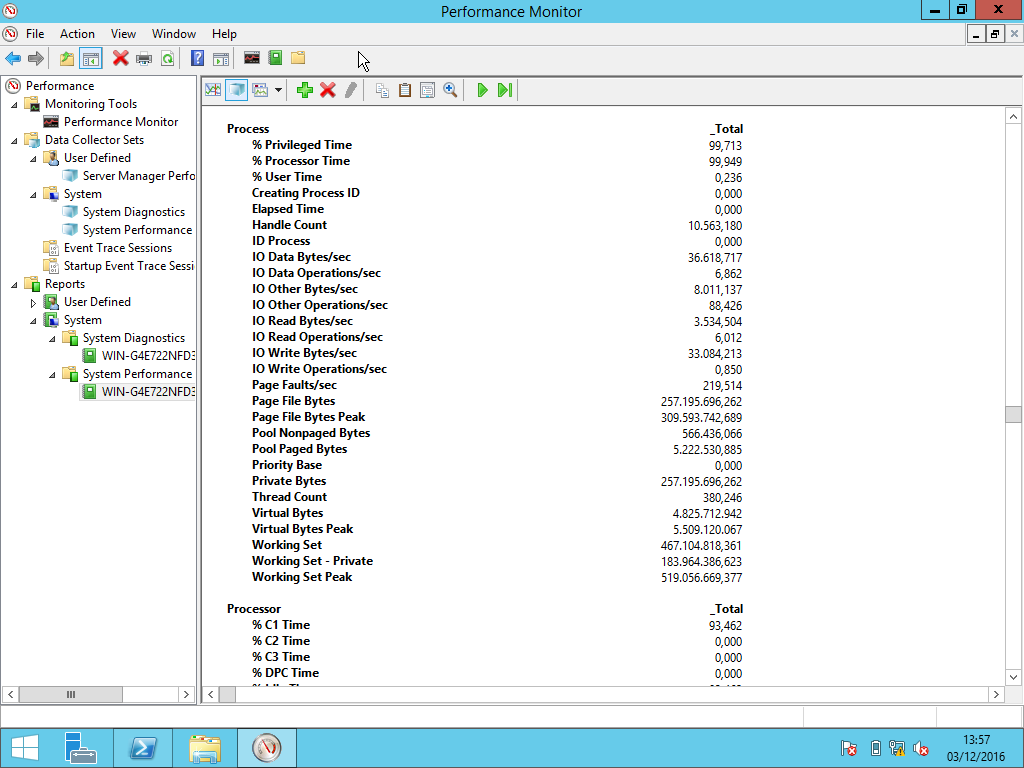
\includegraphics[width=0.7\textwidth]{Imagenes/Datos_grafico_diagnostico_2}
		\caption{Datos sobre los procesos recopilados.} \label{fig:12}
	\end{center}
\end{figure}

Por último mostramos información sobre el procesador, el porcentaje de cada procesador, el porcentaje ocioso, interrupciones por segundo, etc.
\begin{figure}[H]
	\begin{center}
		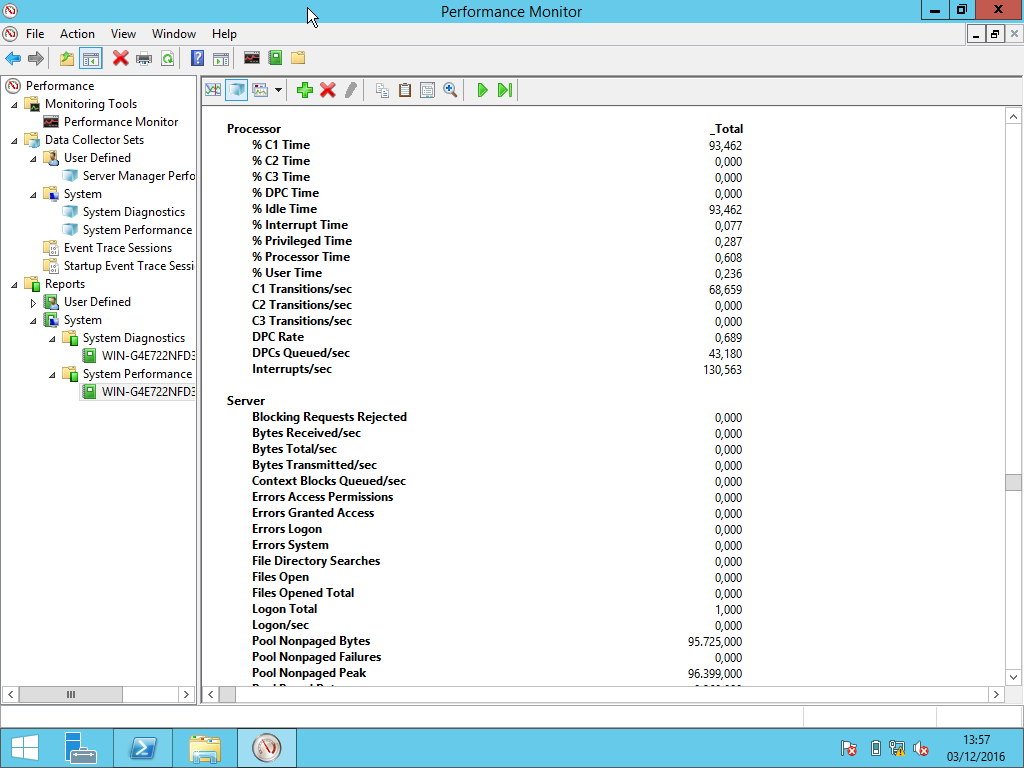
\includegraphics[width=0.7\textwidth]{Imagenes/Datos_grafico_diagnostico_3}
		\caption{Datos sobre el procesador recopilados.} \label{fig:13}
	\end{center}
\end{figure}

\section{Cree un recopilador de datos definido por el usuario (modo avanzado) que incluya tanto el contador de rendimiento como los datos de seguimiento:\\
Todos los referentes al procesador, al proceso y al servicio web.\\
Intervalo de muestra 15 segundos.\\
Almacene el resultado en el directorio Escritorio/logs.\\
Incluya las capturas de pantalla de cada paso.}
\subsection{Respuesta : }

A continuación se muestra el proceso de creación de un recopilador de datos definido por el usuario\cite{PERFORM} :

\begin{figure}[H]
	\begin{center}
		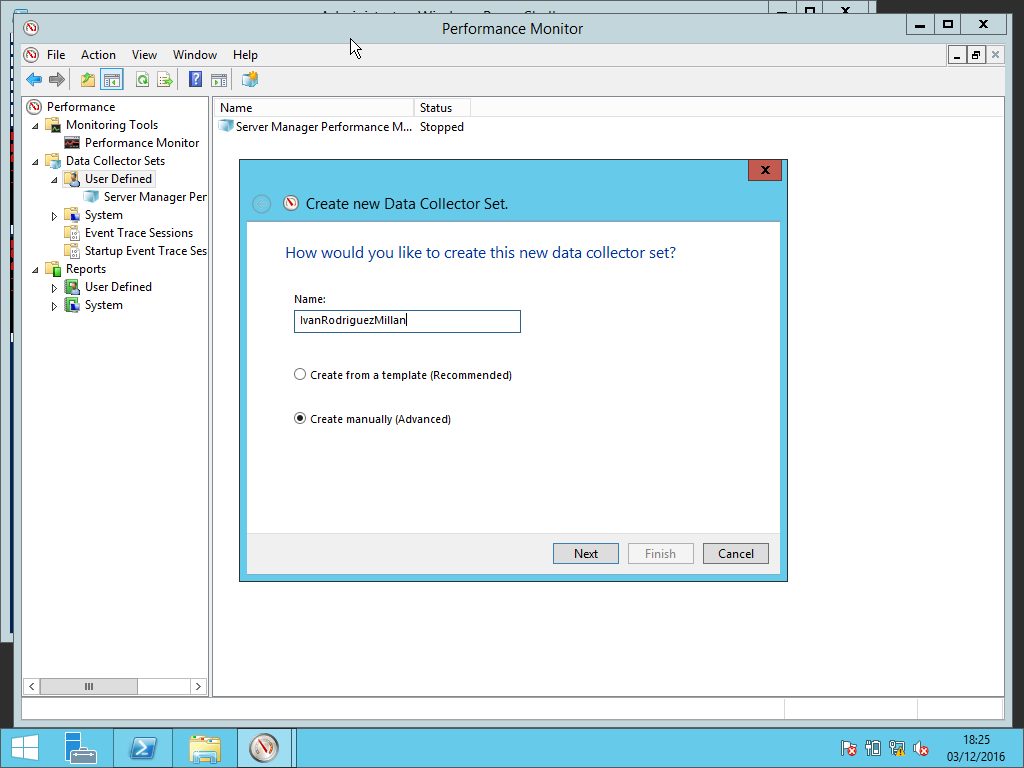
\includegraphics[width=0.7\textwidth]{Imagenes/Inicio_creacion_recopilador_datos}
		\caption{Inicio creación de un recopilador de datos.} \label{fig:14}
	\end{center}
\end{figure}

\begin{figure}[H]
	\begin{center}
		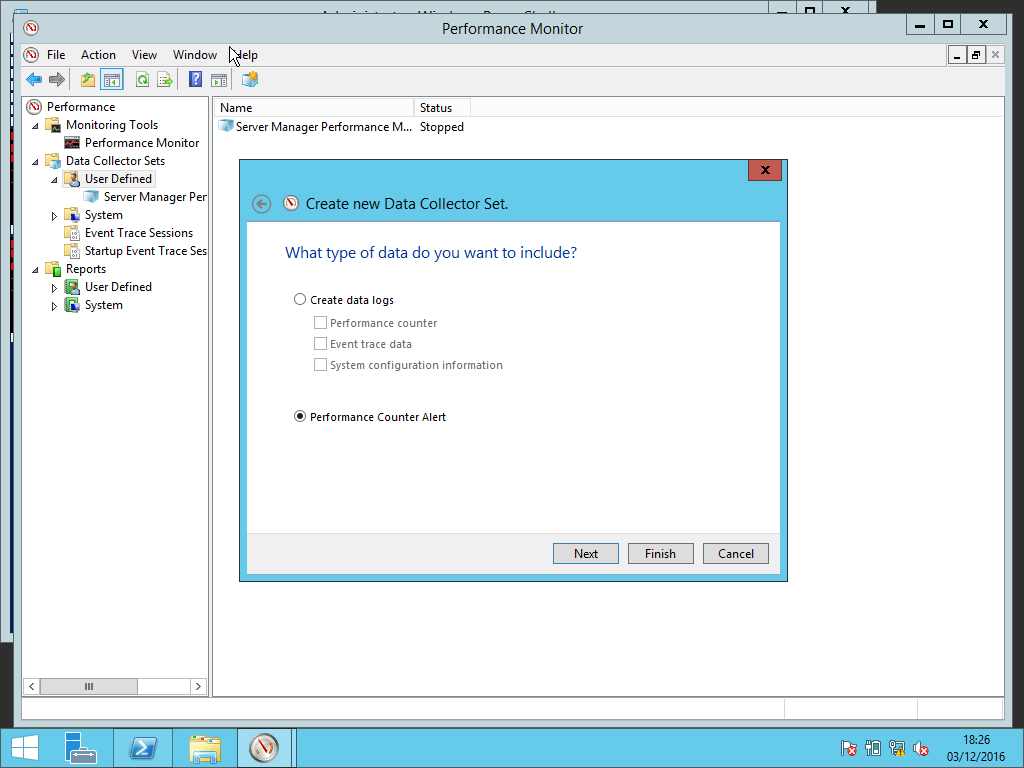
\includegraphics[width=0.7\textwidth]{Imagenes/alerta_contador_rendimiento}
		\caption{Indicando performance counter alert(alerta de contador del rendimiento).} \label{fig:15}
	\end{center}
\end{figure}

\begin{figure}[H]
	\begin{center}
		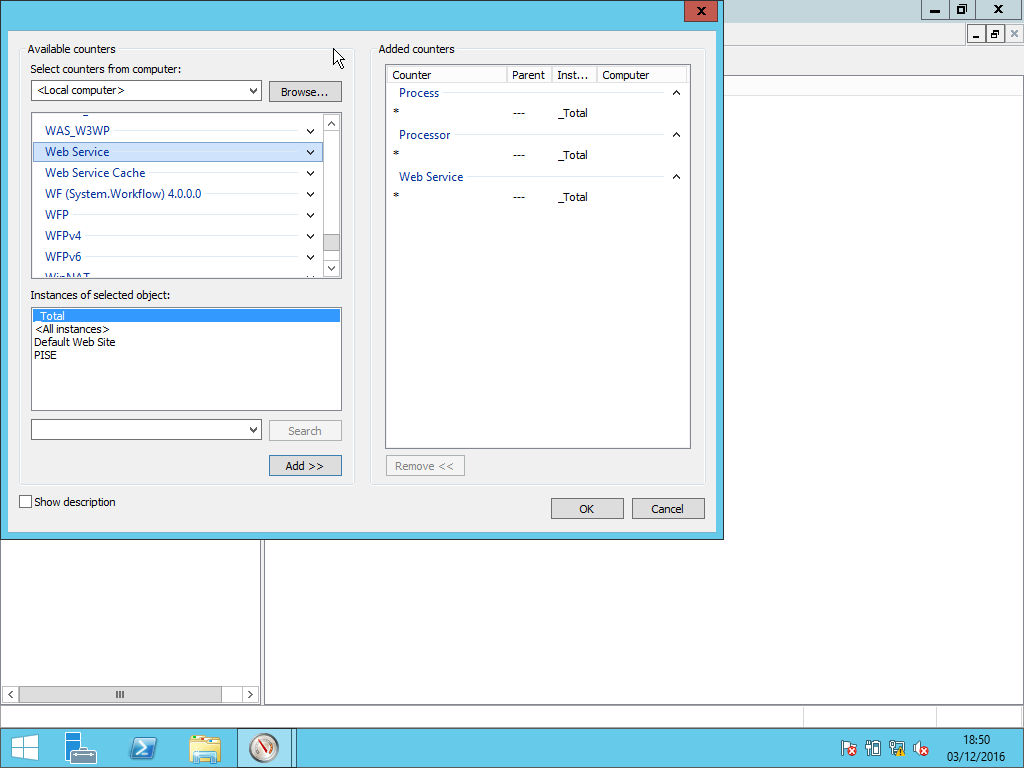
\includegraphics[width=0.7\textwidth]{Imagenes/aniadimos_datos_seguimiento}
		\caption{Añadiendo los contadores de seguimiento , proceso, procesador y servicio web.} \label{fig:16}
	\end{center}
\end{figure}
 
\begin{figure}[H]
	\begin{center}
		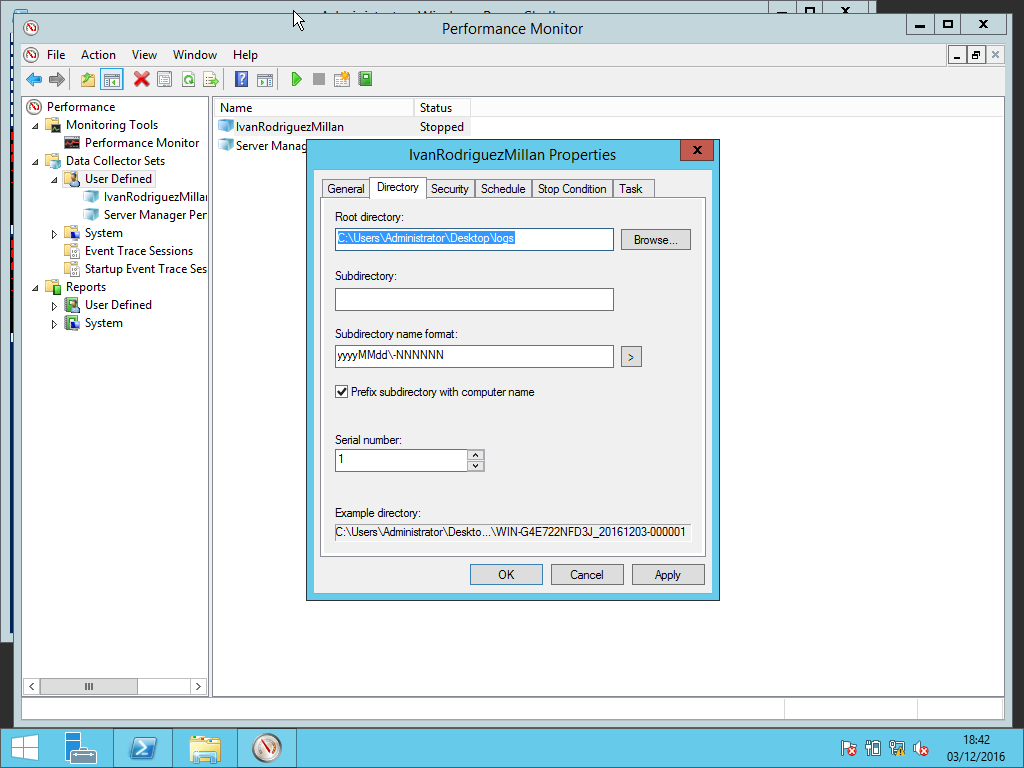
\includegraphics[width=0.7\textwidth]{Imagenes/Cambiando_directorio_almacenamiento}
		\caption{Cambiamos el directorio donde se guardarán los resultados.} \label{fig:17}
	\end{center}
\end{figure}

\begin{figure}[H]
	\begin{center}
		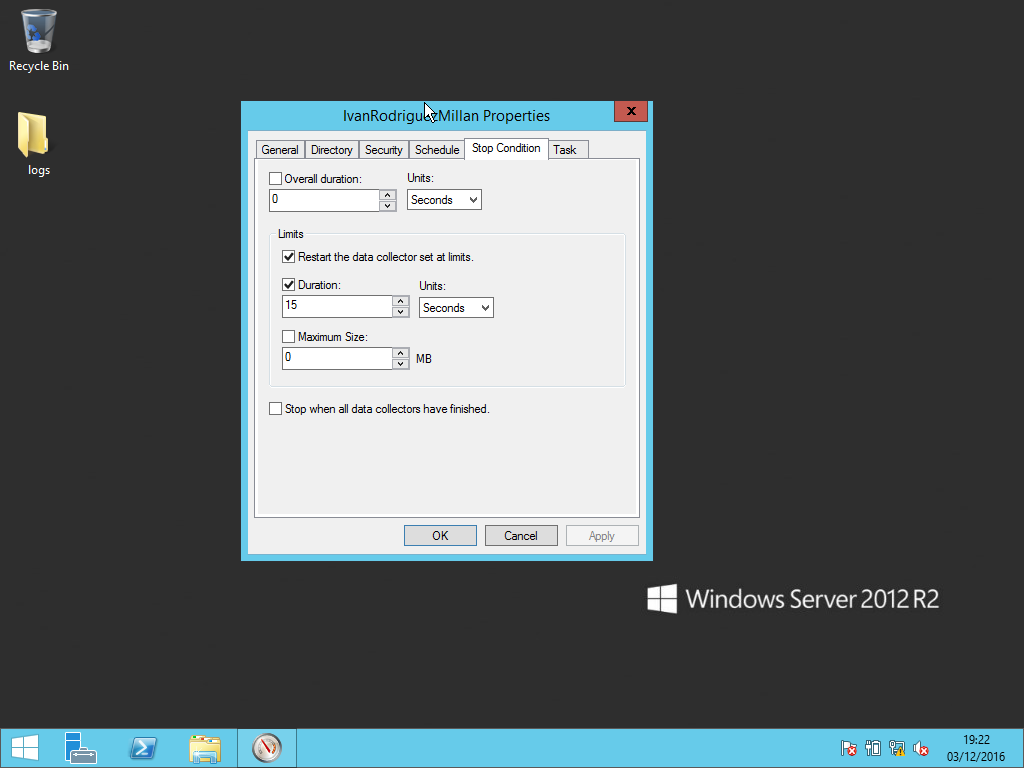
\includegraphics[width=0.7\textwidth]{Imagenes/Limite_reinicio_recopilador}
		\caption{Indicamos que los intervalos de muestras sean cada 15 segundo.} \label{fig:18}
	\end{center}
\end{figure}
\newpage
\section{Visite la web (MUNIN) del proyecto y acceda a la demo que proporcionan donde se muestra cómo monitorizan un servidor. Monitorice varios parámetros y haga capturas de pantalla de lo que está mostrando comentando qué observa.}
\subsection{Respuesta : }

En primer lugar muestro una imagen con la monitorización de la utilización de disco de la última semana. Se puede apreciar como a lo largo de la semana apenas supera el 0 porciento de utilización de disco, salvo el domingo en donde se aprecia un pico de más de un 10 porciento de utilización.

\begin{figure}[H]
	\begin{center}
		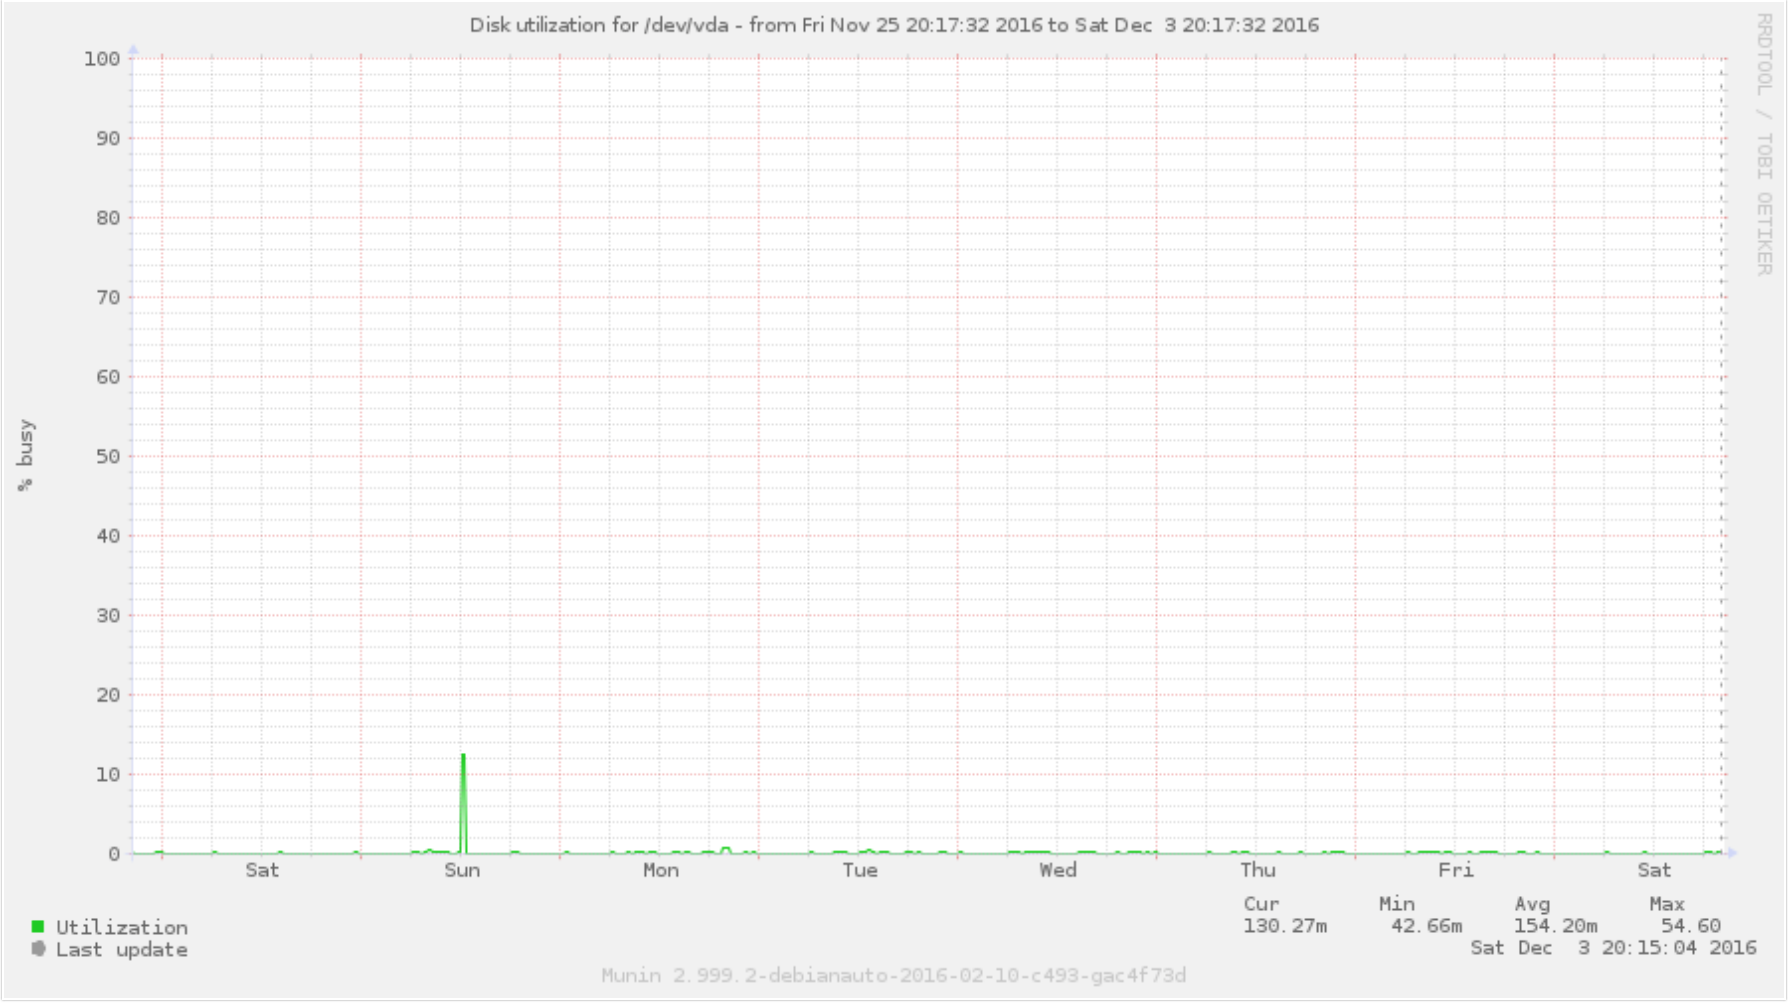
\includegraphics[width=0.7\textwidth]{Imagenes/Monitorizacion_utilizacion_disco}
		\caption{Monitorización de la utilización de disco de la última semana.} \label{fig:19}
	\end{center}
\end{figure}

En segundo lugar se muestra una imagen sobre el uso de CPU en la última semana. En ella se puede apreciar como la mayor parte del tiempo ha estado ociosa, el sistema apenas ha hecho uso, y el usuario/consumidor apenas ha llegado al 20 porciento de uso.
\begin{figure}[H]
	\begin{center}
		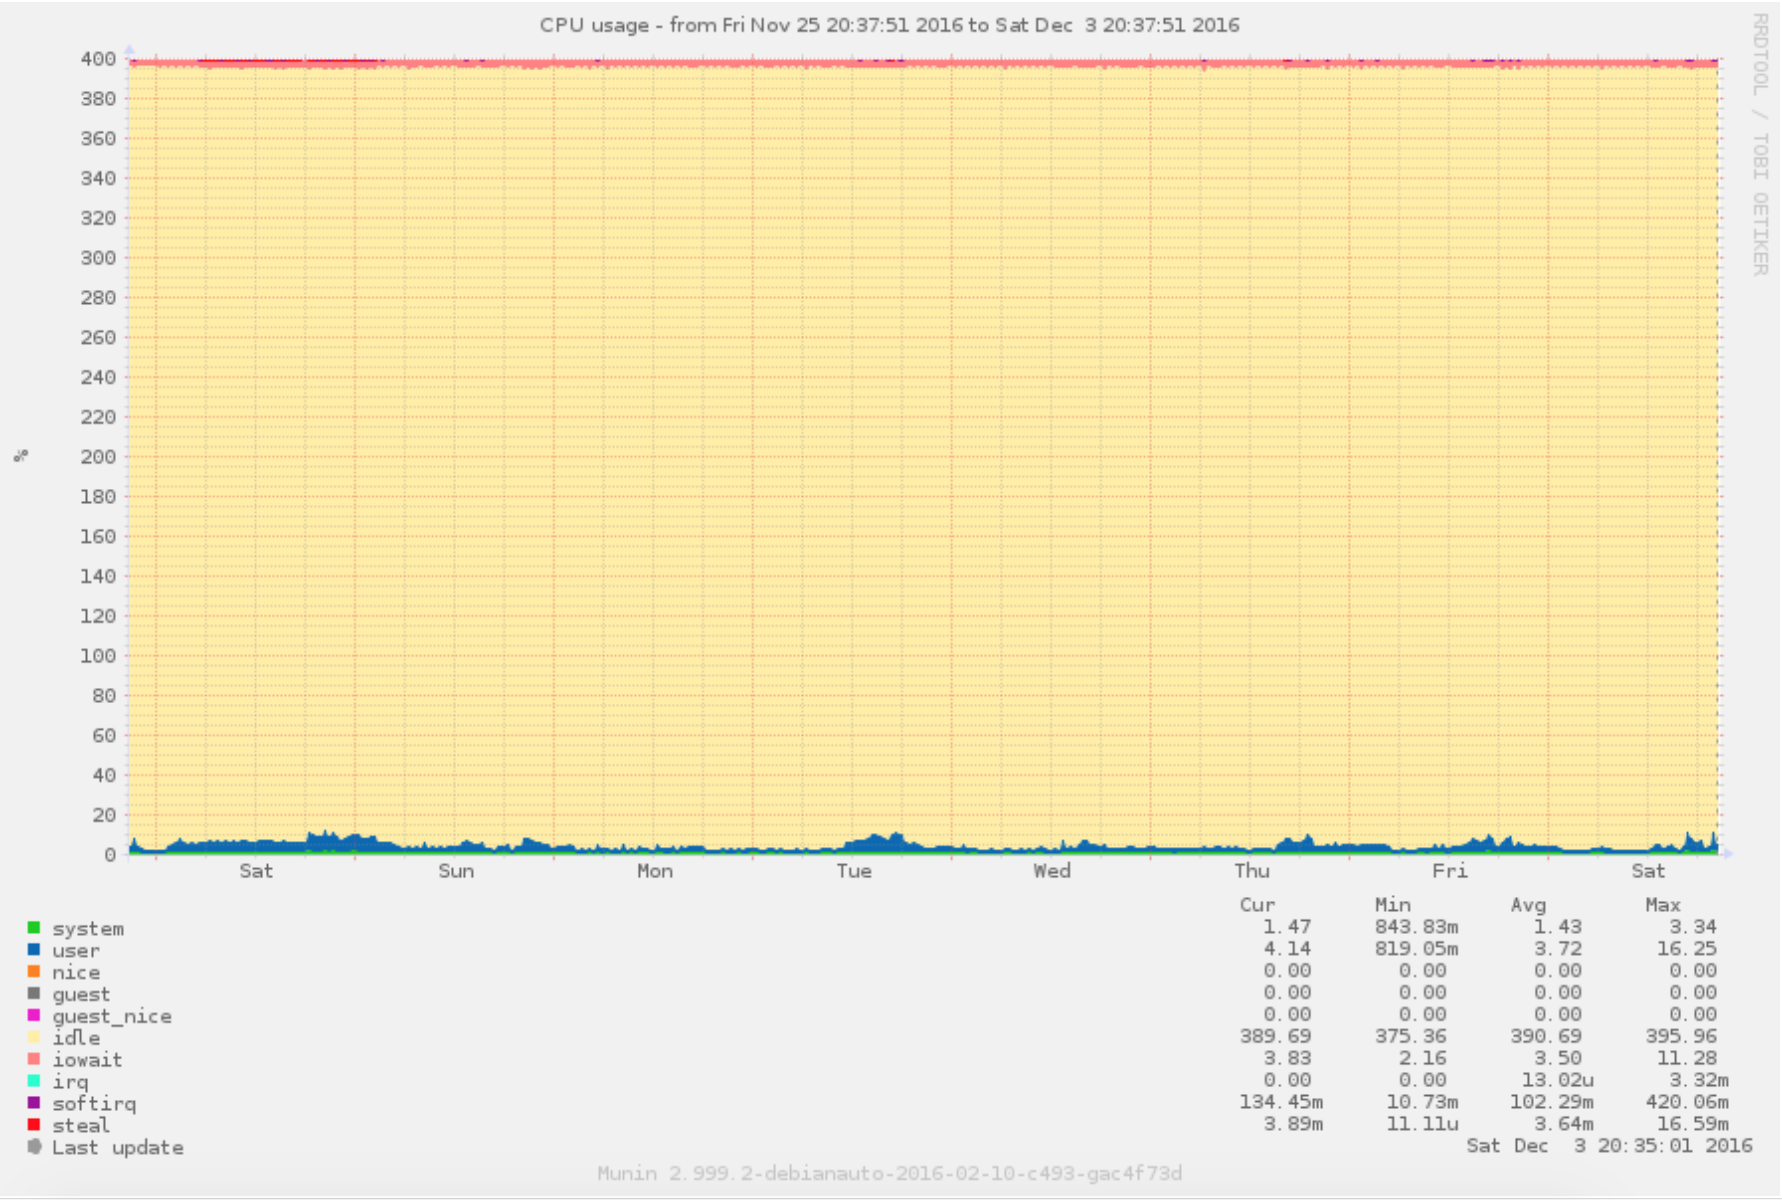
\includegraphics[width=0.7\textwidth]{Imagenes/Monitorizacion_uso_cpu}
		\caption{Monitorización del uso de la CPU de la última semana.} \label{fig:20}
	\end{center}
\end{figure}

En tercer lugar se muestra una imagen con los cambios de contexto e interrupciones producidas en la última semana. Podemos ver como a lo largo de la semana se producen de media unas 131.14 interrupciones y unos 141.09 cambios de contexto de media. Aunque el domingo apreciamos un gran pico de interrupciones llegando desde las 100 hasta las 600, y en cambios de contexto desde los 100 hasta los 1300.

\begin{figure}[H]
	\begin{center}
		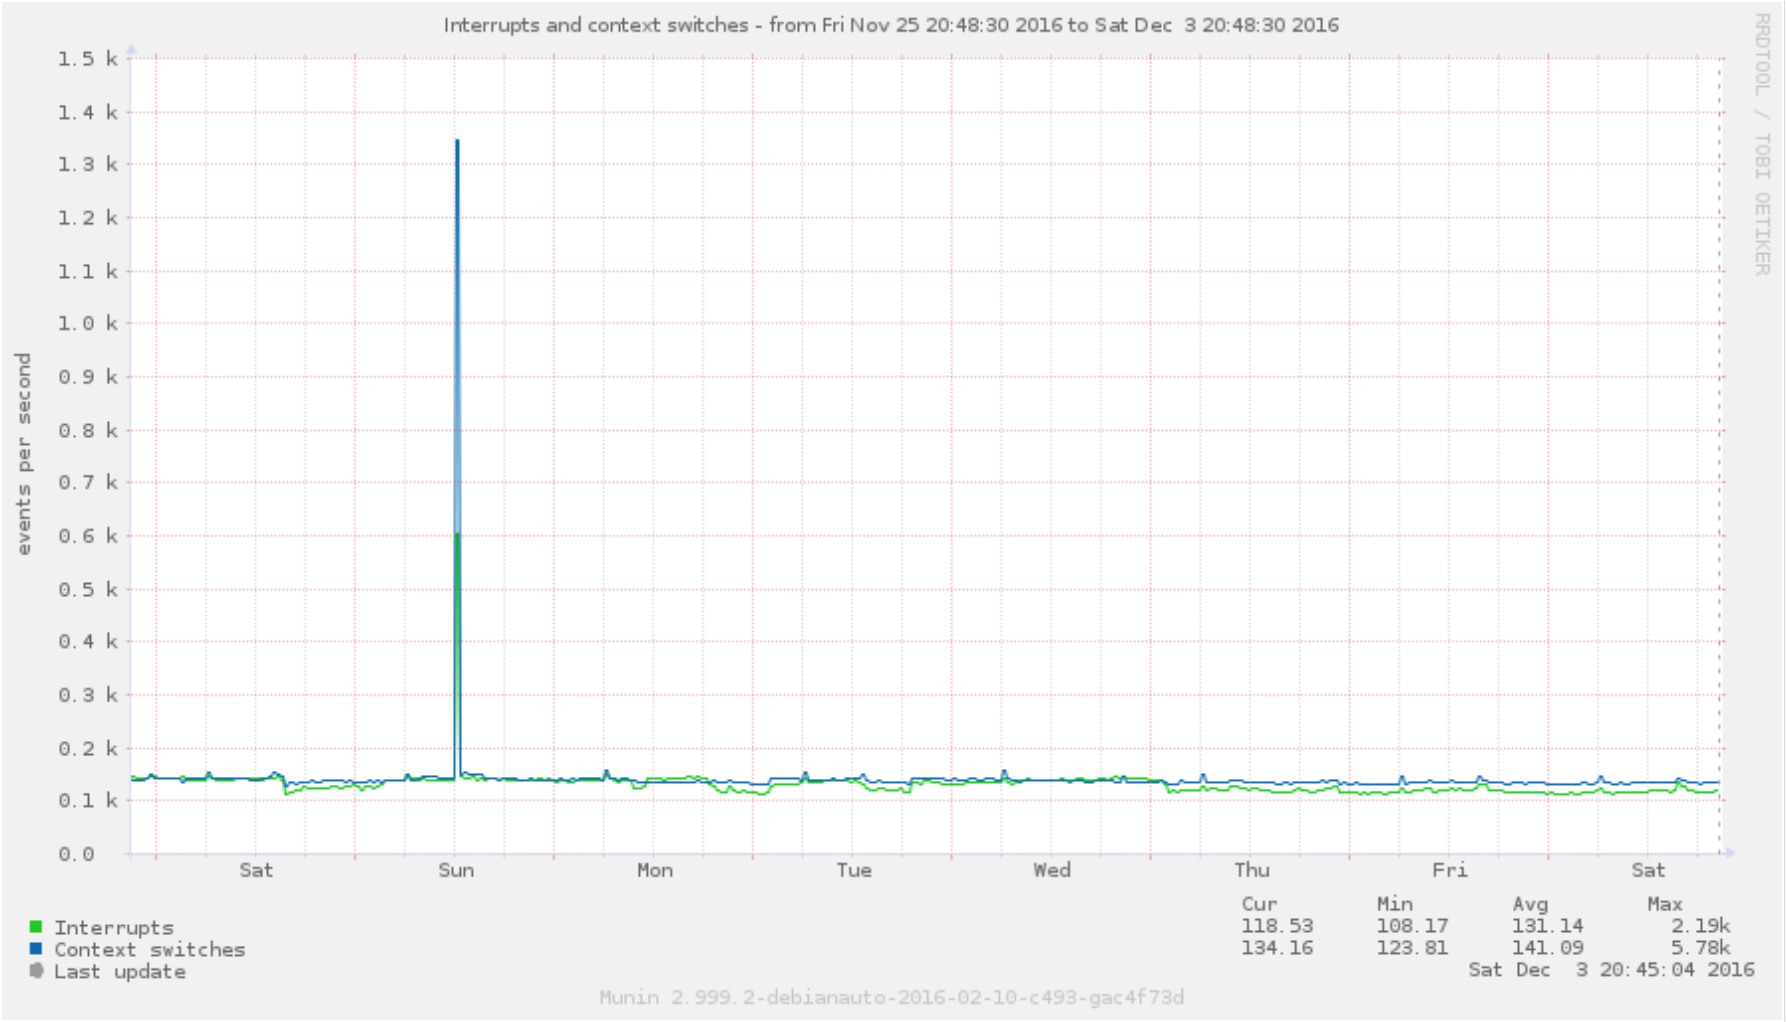
\includegraphics[width=0.7\textwidth]{Imagenes/Monitorizacion_cambios_contexto_interrupciones}
		\caption{Monitorización de los cambios de contexto e interrupciones producidos en la última semana.} \label{fig:21}
	\end{center}
\end{figure}

Y por cuarto lugar muestro una imagen del tráfico en las diferentes interfaces de red(local y eth0). Se ve como de media la interfaz eth0 es por la que más bytes por segundo se envían, y por la interfaz local es por la que más bytes por segundo se reciben. Curiosamente cuando más datos se envían por a través de la interfaz eth0 es en el mes de Diciembre (Concretamente a finales), esto puede ser debido a ser los días de fin de año. También a comienzos de año (Enero y Febrero) se ve un gran aumento de la actividad con respecto al resto de año.
\begin{figure}[H]
	\begin{center}
		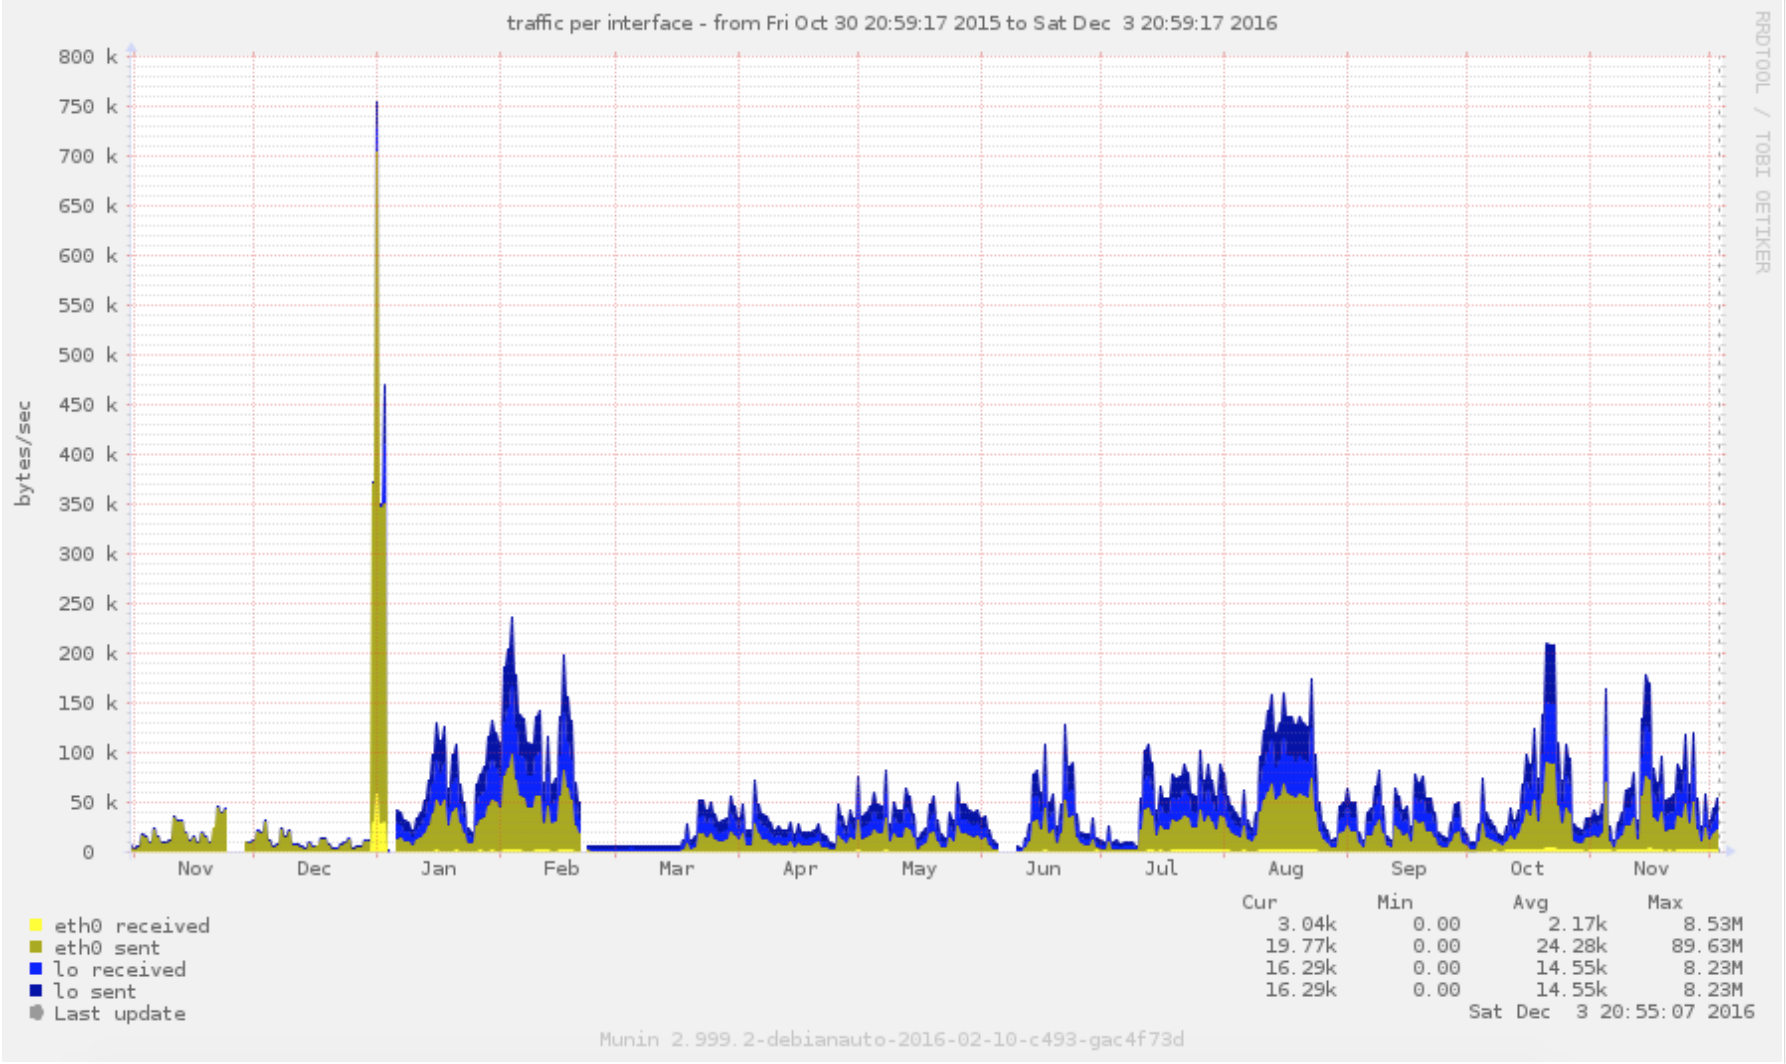
\includegraphics[width=0.7\textwidth]{Imagenes/Monitorizacion_interfaz_de_red}
		\caption{Monitorización del tráfico de bytes por segundo a través de las diferentes interfaces de red en el último año.} \label{fig:22}
	\end{center}
\end{figure}
\section{Escriba un breve resumen sobre alguno de los artículos donde se muestra el uso de strace o busque otro y coméntelo.}
\subsection{Respuesta : }
Muy a menudo ocurre que los procesos finalizan de manera incorrecta y no se tiene información de que problema hubo, ni tampoco información útil de como resolver los errores. Para los administradores de Ubuntu hay una solución, y esta es strace. Strace te muestra lo que el programa está haciendo internamente en cada paso.\\
\newline
Aunque pueda parecer un depurador, no lo es. Y tampoco es una herramienta del programador. Es una herramienta del sistema que sirve para supervisar y visualizar las llamadas y señales del sistema. El uso de strace se lleva a cabo mediante comandos del bash. El uso se hace bastante sencillo, pues solamente tendras que adjuntar strace al proceso, y automáticamente se te mostraran las llamadas del sistema y señales resultantes del proceso.\\
\newline
Vamos a realizar una prueba bastante sencilla de entender. Nos creamos un fichero de texto, y probamos realizar un cat fichero.txt con strace, pero a su vez, para ver las diferencias de cuando nos da error a cuando no, en un caso vamos a tener permisos de lectura y en otro caso no.

\begin{figure}[H]
	\begin{center}
		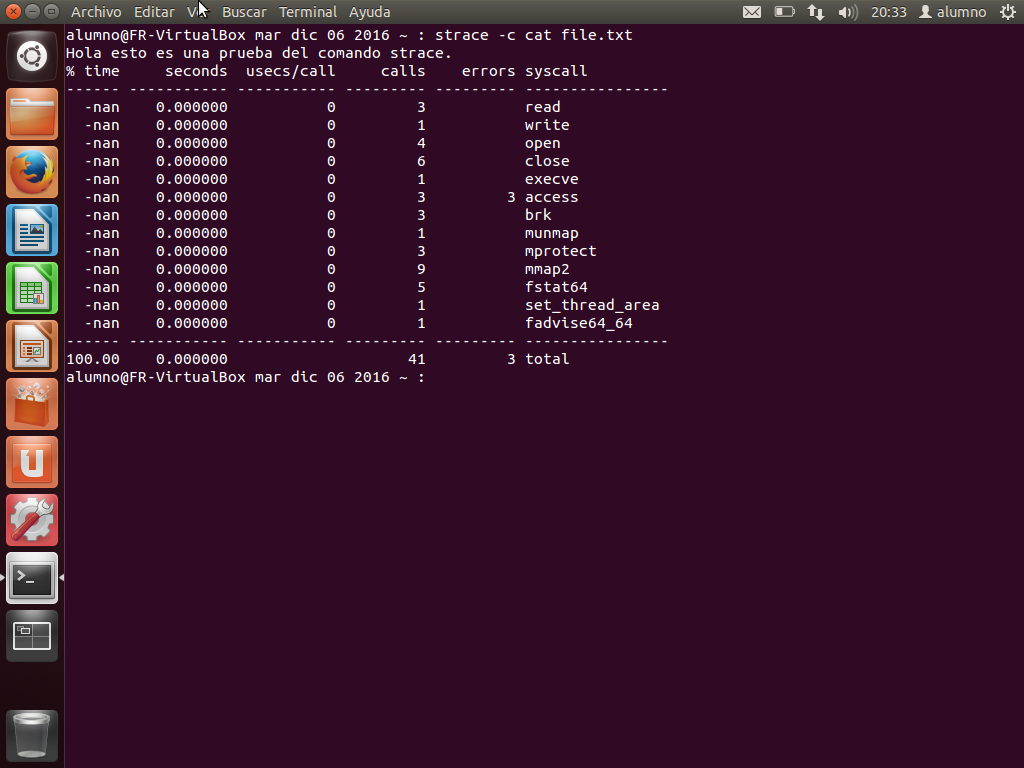
\includegraphics[width=0.7\textwidth]{Imagenes/strace_con_permisos}
		\caption{Ejecución del comando strace teniendo permisos de lectura sobre el fichero de prueba.} \label{fig:23}
	\end{center}
\end{figure}

En el primer caso tenemos permisos de lectura y vemos que en la fila de open no nos da ningún error. Lo ejecutamos con el comando -c, para resumir la información saliente, ya que si lo hiciésemos de la forma tradicional (sin el comando -c), nos saldría una cantidad de información que para el ejemplo es innecesaria.

\begin{figure}[H]
	\begin{center}
		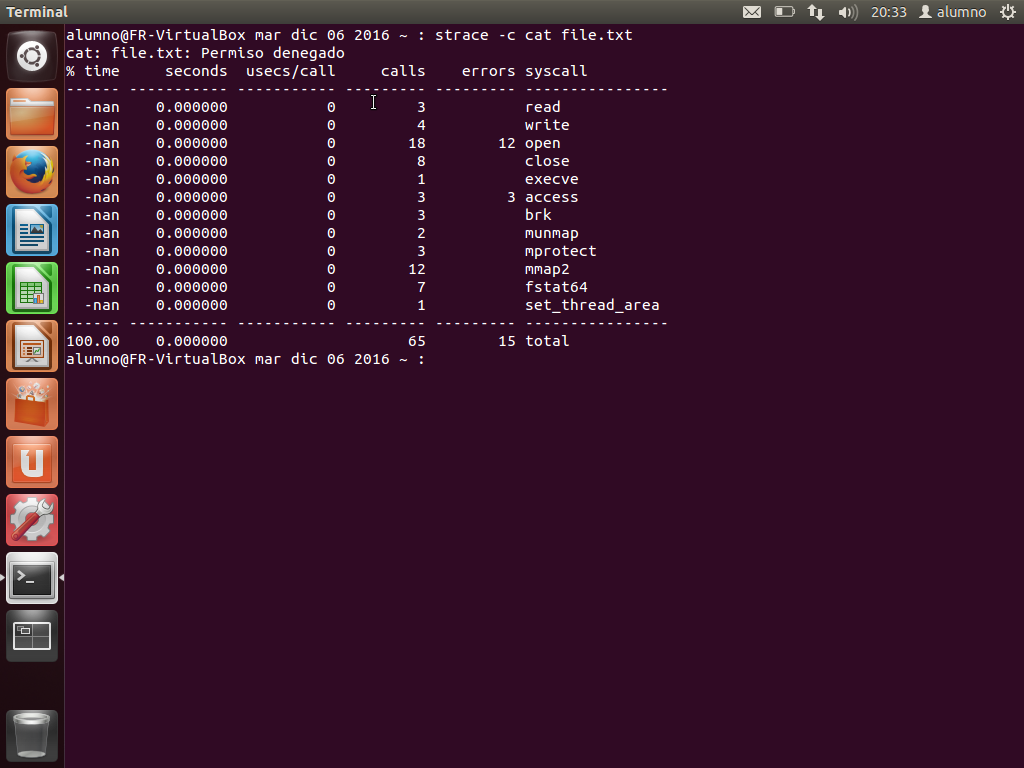
\includegraphics[width=0.7\textwidth]{Imagenes/strace_sin_permisos}
		\caption{Ejecución del comando strace sin tener permisos de lectura sobre el fichero de prueba.} \label{fig:23}
	\end{center}
\end{figure}

En el segundo caso probamos a quitarle permisos de lectura, y efectivamente nos salta con un error en la fila de open. Y es que no podemos abrir un fichero si sobre el no tenemos permisos.
\newpage

\section{Escriba un script en Python o PHP y analice su comportamiento usando el profiler presentado.}
\subsection{Respuesta : }
En mi caso, voy a realizar lo siguiente, en primer lugar, creamos un script para calcular cualquier número de Fibonacci de manera recursiva, y a esto le pasaremos el profiler mencionado en \cite{PYTHON}, seguidamente creamos otro script para calcular cualquier número de Fibonacci también, pero esta vez de manera iterativa. Es conocido el hecho de que el algoritmo de Fibonacci es más rápido de forma iterativa que de forma recursiva debido a la acción de ir guardando los valores anteriores al número a calcular. Así nos deben de dar tiempos bastante dispares para un valor de fibonacci medianamente alto como es el 40 (en Fibonacci el 102334155).

\begin{figure}[H]
	\begin{center}
		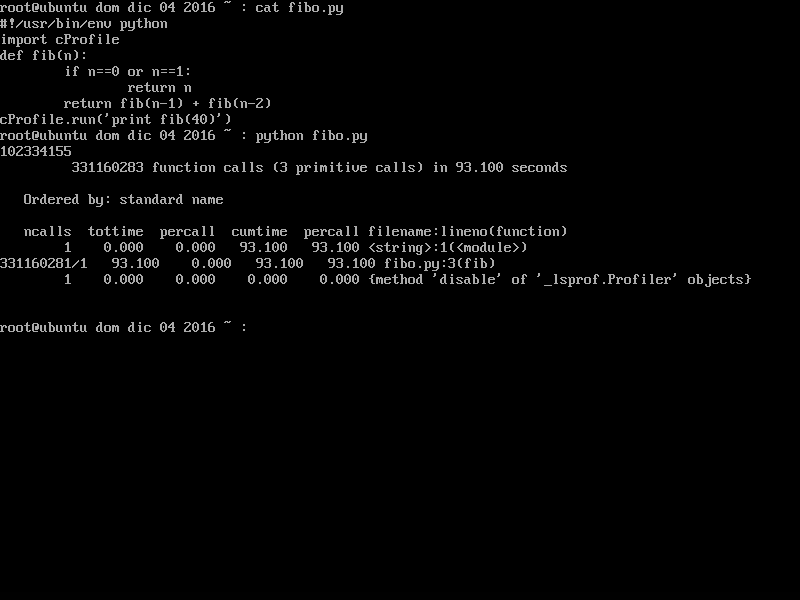
\includegraphics[width=0.7\textwidth]{Imagenes/Fibonacci_recursivo}
		\caption{Analizando el comportamiento de un script recursivo realizado en Python con el profiler cProfiler.} \label{fig:25}
	\end{center}
\end{figure}

En esta imagen, en la salida que proporciona el profiler cProfiler se pueden apreciar varias cosas, en primer lugar, se indica que 331160283 llamadas fueron monitorizadas, y del total 3 fueron primitivas. En total el programa duró 93.1 segundos. 
ncalls es el número de llamadas que se realizan al programa en cuestión, cuando aparecen dos números, viene a indicarnos recursividad en el programa, siendo el segundo valor el número de llamadas primitivas. 
tottime es el tiempo total que se le ha dedicado a la función dada.
percall es el tottime dividido entre ncalls.
cumtime es el tiempo acumulado en la función dada y las funciones inferiores.
Y el último percall es el cociente de cumtime entre las llamadas primitivas.

En la siguiente imagen se muestra lo mismo pero de forma iterativa.

\begin{figure}[H]
	\begin{center}
		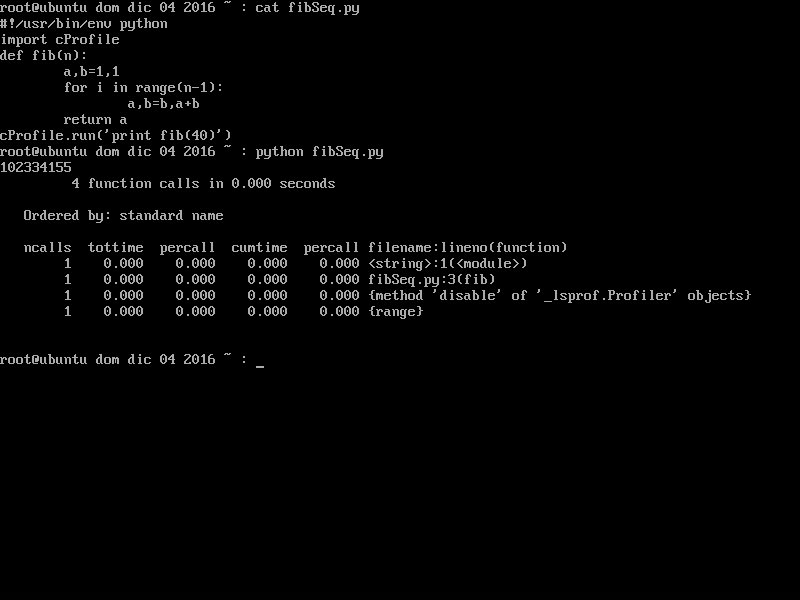
\includegraphics[width=0.7\textwidth]{Imagenes/Fibonacci_iterativo}
		\caption{Analizando el comportamiento de un script iterativo realizado en Python con el profiler cProfiler.} \label{fig:26}
	\end{center}
\end{figure}

En este caso vemos que se monitorizan 4 llamadas, y duraron 0 segundos (Obviamente no duró 0 segundos, simplemente el programa aproxima a 0 el valor que parece haber sido ínfimo).

Se puede apreciar la diferencia claramente entre ambos script y sobre todo la forma de programar un mismo problema como es el de Fibonacci tardando en el primero algo más de 1 minuto y medio, mientras que en el segundo apenas tarda en calcular el valor final.
\newpage
\section{Acceda a la consola mysql (o a través de phpMyAdmin) y muestre el resultado de mostrar el ``profile'' de una consulta (la creación de la BD y la consulta la puede hacer libremente).}
\subsection{Respuesta : }
En primer lugar entramos a mysql y creamos una nueva base de datos \cite{CREARBASEDATOSmysql} para realizar el ejercicio.

\begin{figure}[H]
	\begin{center}
		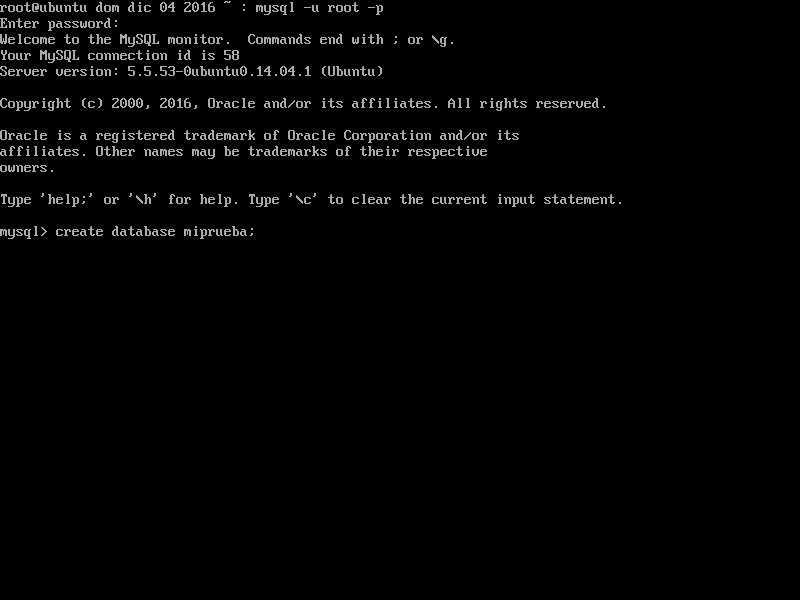
\includegraphics[width=0.7\textwidth]{Imagenes/Acceso_mysql_y_creacion_base_datos}
		\caption{Acceso a mysql y creación de una nueva base de datos.} \label{fig:27}
	\end{center}
\end{figure}

En segundo lugar nos colocamos en esa base de datos con el comando ``use'' , creamos una tabla \cite{CREARTABLAmysql} de prueba e insertamos unos datos. \cite{INSERTARDATOSmysql}

\begin{figure}[H]
	\begin{center}
		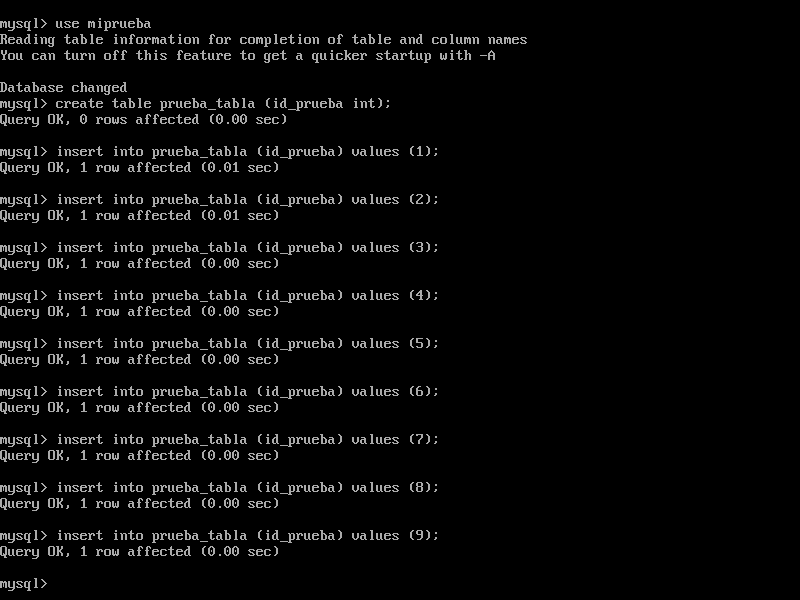
\includegraphics[width=0.7\textwidth]{Imagenes/Seleccion_basedatos_insercion_datos}
		\caption{Creación de una tabla de prueba e inserción de datos.} \label{fig:28}
	\end{center}
\end{figure}

\begin{figure}[H]
	\begin{center}
		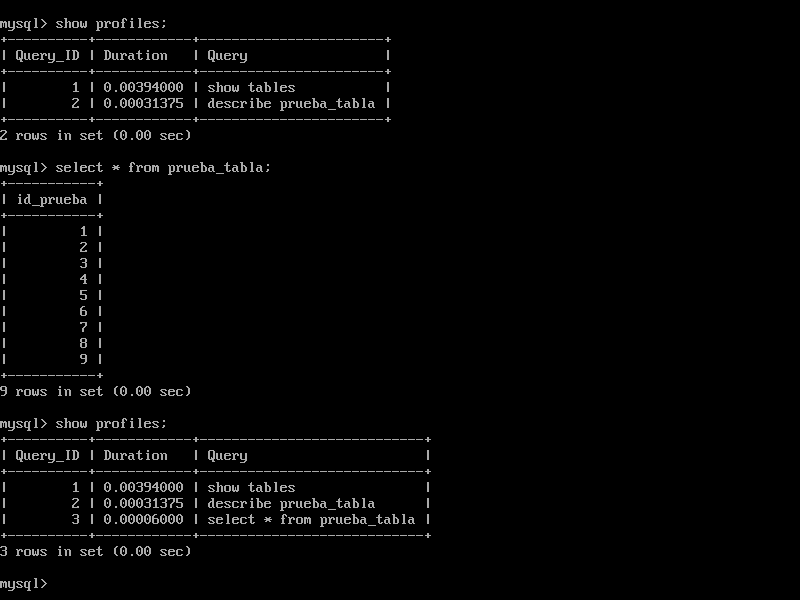
\includegraphics[width=0.7\textwidth]{Imagenes/Verificando_numero_de_consulta}
		\caption{Verificación del número perteneciente a la consulta realizada, para mostrar el profile.} \label{fig:29}
	\end{center}
\end{figure}
\newpage
Y por ultimo realizamos una consulta \cite{CONSULTAmysql} a esta tabla y usando el comando ``show profiles'' verificamos que número se le a asignado a esta consulta, para posteriormente mostrar el profile.

\begin{figure}[H]
	\begin{center}
		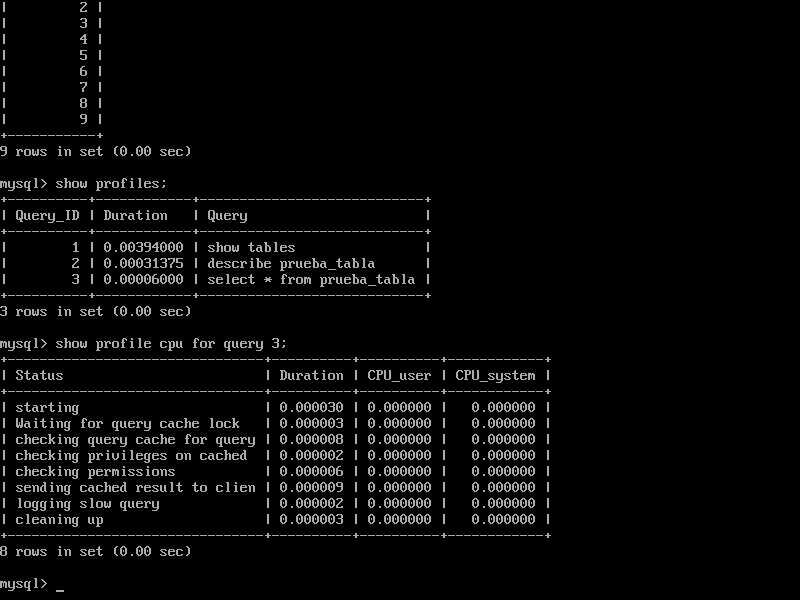
\includegraphics[width=0.7\textwidth]{Imagenes/Profile_aplicado_a_consulta}
		\caption{Mostrando el profile de una consulta realizada a la base de datos creada como ejemplo.} \label{fig:30}
	\end{center}
\end{figure}


\newpage
\bibliography{citas} %archivo citas.bib que contiene las entradas 
\bibliographystyle{ieeetr} % hay varias formas de citar

\end{document}
